% Options for packages loaded elsewhere
\PassOptionsToPackage{unicode}{hyperref}
\PassOptionsToPackage{hyphens}{url}
\documentclass[
  american,
  man, donotrepeattitle,floatsintext]{apa7}
\usepackage{xcolor}
\usepackage{amsmath,amssymb}
\setcounter{secnumdepth}{5}
\usepackage{iftex}
\ifPDFTeX
  \usepackage[T1]{fontenc}
  \usepackage[utf8]{inputenc}
  \usepackage{textcomp} % provide euro and other symbols
\else % if luatex or xetex
  \usepackage{unicode-math} % this also loads fontspec
  \defaultfontfeatures{Scale=MatchLowercase}
  \defaultfontfeatures[\rmfamily]{Ligatures=TeX,Scale=1}
\fi
\usepackage{lmodern}
\ifPDFTeX\else
  % xetex/luatex font selection
\fi
% Use upquote if available, for straight quotes in verbatim environments
\IfFileExists{upquote.sty}{\usepackage{upquote}}{}
\IfFileExists{microtype.sty}{% use microtype if available
  \usepackage[]{microtype}
  \UseMicrotypeSet[protrusion]{basicmath} % disable protrusion for tt fonts
}{}
\makeatletter
\@ifundefined{KOMAClassName}{% if non-KOMA class
  \IfFileExists{parskip.sty}{%
    \usepackage{parskip}
  }{% else
    \setlength{\parindent}{0pt}
    \setlength{\parskip}{6pt plus 2pt minus 1pt}}
}{% if KOMA class
  \KOMAoptions{parskip=half}}
\makeatother
% Make \paragraph and \subparagraph free-standing
\makeatletter
\ifx\paragraph\undefined\else
  \let\oldparagraph\paragraph
  \renewcommand{\paragraph}{
    \@ifstar
      \xxxParagraphStar
      \xxxParagraphNoStar
  }
  \newcommand{\xxxParagraphStar}[1]{\oldparagraph*{#1}\mbox{}}
  \newcommand{\xxxParagraphNoStar}[1]{\oldparagraph{#1}\mbox{}}
\fi
\ifx\subparagraph\undefined\else
  \let\oldsubparagraph\subparagraph
  \renewcommand{\subparagraph}{
    \@ifstar
      \xxxSubParagraphStar
      \xxxSubParagraphNoStar
  }
  \newcommand{\xxxSubParagraphStar}[1]{\oldsubparagraph*{#1}\mbox{}}
  \newcommand{\xxxSubParagraphNoStar}[1]{\oldsubparagraph{#1}\mbox{}}
\fi
\makeatother
\usepackage{graphicx}
\makeatletter
\newsavebox\pandoc@box
\newcommand*\pandocbounded[1]{% scales image to fit in text height/width
  \sbox\pandoc@box{#1}%
  \Gscale@div\@tempa{\textheight}{\dimexpr\ht\pandoc@box+\dp\pandoc@box\relax}%
  \Gscale@div\@tempb{\linewidth}{\wd\pandoc@box}%
  \ifdim\@tempb\p@<\@tempa\p@\let\@tempa\@tempb\fi% select the smaller of both
  \ifdim\@tempa\p@<\p@\scalebox{\@tempa}{\usebox\pandoc@box}%
  \else\usebox{\pandoc@box}%
  \fi%
}
% Set default figure placement to htbp
\def\fps@figure{htbp}
\makeatother
% definitions for citeproc citations
\NewDocumentCommand\citeproctext{}{}
\NewDocumentCommand\citeproc{mm}{%
  \begingroup\def\citeproctext{#2}\cite{#1}\endgroup}
\makeatletter
 % allow citations to break across lines
 \let\@cite@ofmt\@firstofone
 % avoid brackets around text for \cite:
 \def\@biblabel#1{}
 \def\@cite#1#2{{#1\if@tempswa , #2\fi}}
\makeatother
\newlength{\cslhangindent}
\setlength{\cslhangindent}{1.5em}
\newlength{\csllabelwidth}
\setlength{\csllabelwidth}{3em}
\newenvironment{CSLReferences}[2] % #1 hanging-indent, #2 entry-spacing
 {\begin{list}{}{%
  \setlength{\itemindent}{0pt}
  \setlength{\leftmargin}{0pt}
  \setlength{\parsep}{0pt}
  % turn on hanging indent if param 1 is 1
  \ifodd #1
   \setlength{\leftmargin}{\cslhangindent}
   \setlength{\itemindent}{-1\cslhangindent}
  \fi
  % set entry spacing
  \setlength{\itemsep}{#2\baselineskip}}}
 {\end{list}}
\usepackage{calc}
\newcommand{\CSLBlock}[1]{\hfill\break\parbox[t]{\linewidth}{\strut\ignorespaces#1\strut}}
\newcommand{\CSLLeftMargin}[1]{\parbox[t]{\csllabelwidth}{\strut#1\strut}}
\newcommand{\CSLRightInline}[1]{\parbox[t]{\linewidth - \csllabelwidth}{\strut#1\strut}}
\newcommand{\CSLIndent}[1]{\hspace{\cslhangindent}#1}
\ifLuaTeX
\usepackage[bidi=basic,shorthands=off,]{babel}
\else
\usepackage[bidi=default,shorthands=off,]{babel}
\fi
\ifLuaTeX
  \usepackage{selnolig} % disable illegal ligatures
\fi
\setlength{\emergencystretch}{3em} % prevent overfull lines
\providecommand{\tightlist}{%
  \setlength{\itemsep}{0pt}\setlength{\parskip}{0pt}}
% Manuscript styling
\usepackage{upgreek}
\captionsetup{font=singlespacing,justification=justified}

% Table formatting
\usepackage{longtable}
\usepackage{lscape}
% \usepackage[counterclockwise]{rotating}   % Landscape page setup for large tables
\usepackage{multirow}		% Table styling
\usepackage{tabularx}		% Control Column width
\usepackage[flushleft]{threeparttable}	% Allows for three part tables with a specified notes section
\usepackage{threeparttablex}            % Lets threeparttable work with longtable

% Create new environments so endfloat can handle them
% \newenvironment{ltable}
%   {\begin{landscape}\centering\begin{threeparttable}}
%   {\end{threeparttable}\end{landscape}}
\newenvironment{lltable}{\begin{landscape}\centering\begin{ThreePartTable}}{\end{ThreePartTable}\end{landscape}}

% Enables adjusting longtable caption width to table width
% Solution found at http://golatex.de/longtable-mit-caption-so-breit-wie-die-tabelle-t15767.html
\makeatletter
\newcommand\LastLTentrywidth{1em}
\newlength\longtablewidth
\setlength{\longtablewidth}{1in}
\newcommand{\getlongtablewidth}{\begingroup \ifcsname LT@\roman{LT@tables}\endcsname \global\longtablewidth=0pt \renewcommand{\LT@entry}[2]{\global\advance\longtablewidth by ##2\relax\gdef\LastLTentrywidth{##2}}\@nameuse{LT@\roman{LT@tables}} \fi \endgroup}

% \setlength{\parindent}{0.5in}
% \setlength{\parskip}{0pt plus 0pt minus 0pt}

% Overwrite redefinition of paragraph and subparagraph by the default LaTeX template
% See https://github.com/crsh/papaja/issues/292
\makeatletter
\renewcommand{\paragraph}{\@startsection{paragraph}{4}{\parindent}%
  {0\baselineskip \@plus 0.2ex \@minus 0.2ex}%
  {-1em}%
  {\normalfont\normalsize\bfseries\itshape\typesectitle}}

\renewcommand{\subparagraph}[1]{\@startsection{subparagraph}{5}{1em}%
  {0\baselineskip \@plus 0.2ex \@minus 0.2ex}%
  {-\z@\relax}%
  {\normalfont\normalsize\itshape\hspace{\parindent}{#1}\textit{\addperi}}{\relax}}
\makeatother

\makeatletter
\usepackage{etoolbox}
\patchcmd{\maketitle}
  {\section{\normalfont\normalsize\abstractname}}
  {\section*{\normalfont\normalsize\abstractname}}
  {}{\typeout{Failed to patch abstract.}}
\patchcmd{\maketitle}
  {\section{\protect\normalfont{\@title}}}
  {\section*{\protect\normalfont{\@title}}}
  {}{\typeout{Failed to patch title.}}
\makeatother

\usepackage{xpatch}
\makeatletter
\xapptocmd\appendix
  {\xapptocmd\section
    {\addcontentsline{toc}{section}{\appendixname\ifoneappendix\else~\theappendix\fi: #1}}
    {}{\InnerPatchFailed}%
  }
{}{\PatchFailed}
\makeatother
\keywords{meta-analysis; dependent effect sizes; selection models; selective reporting; publication bias}
\usepackage{csquotes}
\usepackage{booktabs}
\usepackage{multirow}
\usepackage{multicol}
\usepackage{amsthm}
\newtheorem{thm}{Theorem}
\newtheorem{lem}{Lemma}
\usepackage{amsfonts}
\usepackage{caption}
\usepackage{multirow}
\usepackage{float}
\usepackage{subfig}
\usepackage{longtable}
\usepackage[figuresright]{rotating}
\geometry{twoside=false, top=1in, bottom=1in, left=1in, right=1in}
\usepackage{hyperref}
\hypersetup{hidelinks}
\raggedbottom
\usepackage{setspace}
\AtBeginEnvironment{tabular}{\singlespacing}
\usepackage{perpage}
\MakePerPage{footnote}
\renewcommand{\thefootnote}{\fnsymbol{footnote}}
\usepackage{xr}
\externaldocument{step-function-selection-models-supplementary-materials}
\newcommand{\Prob}{\text{Pr}}
\newcommand{\E}{\text{E}}
\newcommand{\Cov}{\text{Cov}}
\newcommand{\cor}{\text{cor}}
\newcommand{\Var}{\text{Var}}
\newcommand{\diag}{\text{diag}}
\newcommand{\mat}[1]{\mathbf{#1}}
\newcommand{\bs}{\boldsymbol}
\newcommand{\trace}{\text{tr}}
\usepackage{bookmark}
\IfFileExists{xurl.sty}{\usepackage{xurl}}{} % add URL line breaks if available
\urlstyle{same}
\hypersetup{
  pdftitle={Estimation and inference for step-function selection models in meta-analysis with dependent effects},
  pdfauthor={James E. Pustejovsky1, Martyna Citkowicz2, \& Megha Joshi2},
  pdflang={en-US},
  pdfkeywords={meta-analysis; dependent effect sizes; selection models; selective reporting; publication bias},
  hidelinks,
  pdfcreator={LaTeX via pandoc}}

\title{Estimation and inference for step-function selection models in meta-analysis with dependent effects}
\author{James E. Pustejovsky\textsuperscript{1}, Martyna Citkowicz\textsuperscript{2}, \& Megha Joshi\textsuperscript{2}}
\date{}


\shorttitle{Step-function selection models}

\authornote{

Correspondence concerning this article should be addressed to James E. Pustejovsky, 1082C Educational Sciences, 1025 W Johnson St.~Madison, WI 53706-1706. E-mail: \href{mailto:pustejovsky@wisc.edu}{\nolinkurl{pustejovsky@wisc.edu}}

}

\affiliation{\vspace{0.5cm}\textsuperscript{1} University of Wisconsin-Madison\\\textsuperscript{2} American Institutes for Research}

\note{~\newline June 02, 2025}

\abstract{%
Meta-analyses in social science fields face multiple methodological challenges arising from how primary research studies are designed and reported. One challenge is that many primary studies report multiple relevant effect size estimates. Another is selective reporting bias, which arises when the availability of study findings is influenced by the statistical significance of results. Although many selective reporting diagnostics and bias-correction methods have been proposed, few are suitable for meta-analyses involving dependent effect sizes. Among available methods, step-function selection models are conceptually appealing and have shown promise in previous simulations. We study methods for estimating step-function models from data involving dependent effect sizes, focusing specifically on estimating parameters of the marginal distribution of effect sizes and accounting for dependence using cluster-robust variance estimation or bootstrap resampling. We describe two estimation strategies, demonstrate them by re-analyzing data from a synthesis on ego depletion effects, and evaluate their performance through an extensive simulation study under single-step selection. Simulation findings indicate that selection models provide low-bias estimates of average effect size and that clustered bootstrap confidence intervals provide acceptable coverage levels. However, adjusting for selective reporting bias using step-function models involves a bias-variance trade-off, and unadjusted estimates of average effect sizes may be preferable if the strength of selective reporting is mild.
}



\begin{document}
\maketitle

\section{Introduction}\label{introduction}

The validity of conclusions from meta-analytic syntheses depend critically on the reporting practices of researchers, journal editors, and peer reviewers.
If the findings accessible to meta-analysts are not a representative record of the research that has been conducted on a topic, then meta-analytic summaries may be systematically biased.\textsuperscript{1}
Of particular concern is the possibility that results from primary studies are selectively reported in ways that can distort the evidence available for synthesis, such as reporting findings that are statistically significant but omitting findings that are null or not consistent with researchers' hypotheses.\textsuperscript{2}

Evidence from medical, educational, and social sciences provides indications of the prevalence of selective reporting. For example, studies have found that statistically significant outcomes were 2.4 to 4.7 times more likely to be published than non-significant outcomes in the medical sciences\textsuperscript{3} and 2.4 times more likely in education.\textsuperscript{4} Research across various fields, from clinical trials of antipsychotics\textsuperscript{5} to psychology studies\textsuperscript{6,7} and management research\textsuperscript{8}, indicates that selective outcome reporting is widespread and often driven by statistical significance.

Because selective reporting is of such central concern for meta-analysis, a wide range of statistical tools have been developed for assessing the presence of selective reporting and reducing the biases it creates.\textsuperscript{1,9}
One common graphical diagnostic is the funnel plot, a simple scatterplot of effect size estimates versus a measure of their precision.\textsuperscript{10--12} Widely used statistical diagnostics include the rank correlation test\textsuperscript{13}; Egger's regression test\textsuperscript{14--17}; the trim-and-fill adjustment\textsuperscript{18,19}; and various regression adjustment methods including the precision effect test (PET), precision effect estimate with standard error (PEESE), and PET-PEESE technique\textsuperscript{20}, and the endogenous kink meta-regression\textsuperscript{21}.

Another class of methods for assessing and correcting selective reporting are \(p\)-value selection models.
Such models build on summary meta-analysis or meta-regression models by making specific, explicit assumptions about the selection function, or how the probability that an effect size estimate is reported relates to sign and statistical significance level of the effect. Building on earlier proposals\textsuperscript{22--24}, Vevea and Hedges proposed \emph{step-function} models where the selection function is piece-wise constant, with steps at psychologically salient significance levels such as \(\alpha = .05\).\textsuperscript{25,26}
Other forms involve selection functions based on beta densities\textsuperscript{27}, power curves, and a variety of other parametric forms.\textsuperscript{28}

Selection models have several advantages over other available methods for diagnosing and adjusting for selective reporting bias.
First, they are generative models with parameters that directly describe the selective reporting process; they are therefore more interpretable than tests or adjustments for small-study effects, which are agnostic with respect to the specific mechanism of selective reporting.
Second, selection models can allow for effect heterogeneity with a random effect term.
Findings from simulations indicate that selection models outperform simpler alternative methods when effect sizes are heterogeneous.\textsuperscript{2,29}
Third, selection models can incorporate both discrete and continuous moderators, enabling one to distinguish between selective reporting bias and systematic differences in effect size that can be predicted by primary study characteristics.
In addition to these features, the step-function selection model is particularly useful because it allows one to specify cut points that capture simple but plausible forms of selective reporting (e.g., p \textless{} 0.01 and p \textless{} 0.05).\textsuperscript{30--33}

\subsection{Dependent effect sizes}\label{dependent-effect-sizes}

The vast majority of the work on selective reporting has focused on methods appropriate for relatively simple summary meta-analyses in which each included study contributes a single independent effect size estimate.
This presents a problem for syntheses in education, psychology, and many other areas, where meta-analyses routinely include studies with multiple, dependent effect sizes.
Effect size dependencies occur when multiple effect sizes are extracted from the same sample, resulting in statistically dependent estimates.
Dependent effect size estimates commonly occur (1) when multiple outcome measures are collected on the same sample; (2) when the same sample is measured over multiple time points; or (3) when multiple treatment groups are compared to the same control group.\textsuperscript{34}
Dependence can also arise when effect sizes are extracted from multiple samples involving the same operational features, such as multiple studies conducted by the same research group.\textsuperscript{35}

Effect size dependencies are very common in social science synthesis, as well as in other research areas.
For example, for the more than 1,000 educational intervention studies reviewed by the What Works Clearinghouse since 2017, most (73\%) included more than one intervention effect estimate, with a median of four effect sizes per study (WWC, 2020).
Surveys of systematic reviews on topics in psychology and education\textsuperscript{36}, environmental sciences\textsuperscript{37}, and neurobiology\textsuperscript{38} have also documented a high prevalence of dependent effect sizes.
Thus, multiple effects are the norm, rather than the exception, in many fields that use quantitative synthesis.

Meta-analysts now have access to an array of methods for summarizing and modeling dependent effect sizes, including multi-level meta-analyses\textsuperscript{39--41}, robust variance estimation\textsuperscript{RVE, 35}, and combinations thereof\textsuperscript{42}.
Among these, RVE has proven to be an attractive strategy because it provides a means to assess uncertainty in model parameter estimates that does not rely on strong assumptions about the exact dependence structure of the effect size estimates.
Instead, RVE involves specifying a tentative working model for the dependence, but calculating standard errors, hypothesis tests, and confidence intervals using sandwich estimators that do not require the working model to be correct.
Although the original form of RVE required a relatively large number of independent studies, subsequent work has provided refinements to standard errors and hypothesis tests based on RVE to provide accurate inferences even when the number of studies is small.\textsuperscript{43,44}
A closely related strategy is to use bootstrap re-sampling to approximate the distribution of test statistics.\textsuperscript{45}
However, extant developments in RVE and bootstrapping methods are limited to summary meta-analysis and meta-regression models.
Applications to selection models remain to be explored.

\subsection{Investigating selective reporting with dependent effect sizes}\label{investigating-selective-reporting-with-dependent-effect-sizes}

Methodologists have only recently begun to examine selective reporting detection or bias correction methods in meta-analysis involving dependent effect sizes.
Mathur and VanderWeele proposed a sensitivity analysis based on the simplest possible form of the step-function selection model.\textsuperscript{46}
This sensitivity analysis provides an estimate of the average effect size after correcting for selective reporting based on a single, threshold statistical significance level, where the maximum strength of selection is pre-specified by the analyst.
It handles effect size dependence using RVE.\textsuperscript{35}
However, this approach is premised on an assumed degree of selective reporting; thus, it does not estimate the strength of selection, nor does it have extensions to more complex forms of selection models (such as step functions with multiple thresholds).

Another alternative is to use a regression test for small-study effects, or association between effect sizes and standard errors, combined with RVE or multilevel meta-analysis to handle dependent effect sizes.\textsuperscript{47,48}
This method has limited power to detect selective reporting under common meta-analytic scenarios.\textsuperscript{48}
It also has the same limitations as univariate Egger's regression, in that it tests for small-study effects (or asymmetry in the funnel plot distribution), which could have causes other than selective reporting.
Further, Egger's regression is not based on a generative model and is therefore not directly informative about the degree or pattern of selective reporting.

Chen and Pustejovsky reviewed a range of existing techniques for estimating average effect sizes in the presence of selective reporting and proposed adaptations of some existing methods to accommodate dependent effect sizes.\textsuperscript{49}
The proposed adaptations applied to methods that could be formulated as meta-regressions, such as PET/PEESE and the endogenous kink method, with dependence addressed using a particular working model combined with RVE.
In an extensive simulation study, they examined the performance of proposed adaptations alongside existing methods that ignore effect size dependence.
Although no single bias-correction method performed best across all conditions examined, simple forms of the step-function selection model emerged as strong candidates.
Across a wide range of conditions, one-step and two-step selection models yielded average effect size estimates with low bias that were usually more accurate than alternative bias-adjusted estimators, even though the selection models ignore the dependence structure of the data.
However, because selection models rely on the assumption that all effect sizes are independent, confidence intervals generated from the selection models did not have accurate coverage.
These findings indicate a clear need to further develop selection models that can account for dependent effect sizes.\textsuperscript{49}

To address this need, we investigate how to estimate selection models and provide valid assessments of uncertainty in parameter estimates for meta-analyses that involve dependent effect sizes.
In the next section, we describe the step-function selection model and detail two different strategies for estimating model parameters: one using conventional maximum likelihood estimation methods and a novel strategy based on a re-weighted random effects model with inverse probability of selection weights.
We also describe extensions of RVE and bootstrap re-sampling techniques to assess uncertainty in selection model parameter estimate
In the following section, we provide an empirical example that illustrates the methods by re-analyzing data from a previously reported meta-analysis.
In subsequent sections, we describe the methods and results from a simulation study that evaluates the performance of point estimators and confidence intervals across a wide range of meta-analytic conditions.
In the final section, we discuss findings, limitations, and initial implications for practice.

\section{Models and Estimation Methods}\label{model-and-estimation}

Step-function selection models involve two components.\textsuperscript{50}
The first component, which we shall call the evidence-generating process, involves assumptions about the distribution of effect size estimates prior to selective reporting.
This component is usually a random effects model or meta-regression model.
The second component, which we shall call the selection process, involves assumptions about how effect size estimates come to be observed and therefore available for inclusion in the meta-analysis.
Combining the assumptions of both components leads to a model for the distribution of observed effect size estimates, with interpretable parameters describing both the evidence-generating process and the selection process.

In applying selection models to datasets involving dependent effects, we propose to model the \emph{marginal} distribution of the effect size estimates---that is, the distribution of each estimate considered singly---rather than modeling the joint distribution of the multiple observed effects reported in a primary study.
To account for dependence, we consider cluster-robust variance estimation or clustered bootstrap inference methods that allow for dependent observations even though the dependence is not explicitly modeled.
This strategy does have the limitation that the model parameter estimates pertain only to the marginal distribution and do not distinguish between selective publication of full studies versus selective reporting of individual outcomes.
Nonetheless, we believe that the strategy is worth pursuing both because it is feasible and because it captures a plausible form of selection, in which reporting is influenced by the significance level of individual effect size estimates.

We will use the following notation to describe the model and estimation methods. Consider a meta-analytic sample consisting of \(J\) studies, in which study \(j\) reports \(k_j\) effect size estimates. Let \(y_{ij}\) denote observed effect size estimate \(i\) from study \(j\), defined so that positive values are consistent with theoretical expectations. Each estimate is accompanied by a standard error \(\sigma_{ij}\) and corresponding one-sided \(p\)-value \(p_{ij}\), where the one-sided \(p\)-value is defined with respect to the null hypothesis that the effect is less than or equal to zero and the alternative hypothesis that the effect is positive. Let \(\mathbf{x}_{ij}\) be a \(1 \times x\) row-vector of predictors that encode characteristics of the effect sizes, samples, or study procedures. Let \(\Phi()\) denote the standard normal cumulative distribution function and \(\phi()\) denote the standard normal density function.

\subsection{Evidence-generating process}\label{evidence-generating-process}

We consider an evidence-generating process based on a standard meta-regression model.
Let \(Y^*\) denote an effect size estimate that has been generated from primary study data but might or might not be reported; let \(\sigma^*\), \(p^*\), and \(\mathbf{x}^*\) denote the corresponding standard error, one-sided \(p\)-value, and predictor vector.
The evidence-generating process can then be expressed as
\begin{equation}
\label{eq:meta-mean-regression}
\left(Y^* | \sigma^*, \mathbf{x}^*\right) \sim N\left(\mathbf{x}^* \boldsymbol\beta, \ \tau^2 + \sigma^{*2}\right),
\end{equation}
where \(\boldsymbol\beta\) is an \(x \times 1\) vector of regression coefficients that relate the predictors to average effect size and \(\tau^2\) is the variance of the distribution of effect size parameters.
This random-effects meta-regression treats each observed effect size as if it were independent, even though the data may include multiple, statistically dependent effect size estimates generated from the same sample.
As a result, the regression coefficients \(\boldsymbol\beta\) describe the overall expected effect size (given the predictors) and the variance parameter \(\tau^2\) describes the marginal or \emph{total} heterogeneity of the effect size distribution, rather than decomposing the heterogeneity into within-study and between-study components.

\subsection{Selection process}\label{selection-process}

At a general level, a \(p\)-value selection process is defined by a selection function, which specifies the probability that an effect size estimate is reported given its \(p\)-value.
Letting \(O\) be an indicator for whether the effect size estimate \(Y^*\) is observed, the selection process defines \(\text{Pr}(O = 1 \ | \ p^*) = \text{Pr}(O = 1 \ | \ Y^*, \sigma^*)\).
In particular, such models assume that
\(\Pr\left(O = 1 | p^* \right)\) is proportional to a function \(w\left(p^*; \boldsymbol\lambda \right)\) that maps \(p\)-values in the interval \([0,1]\) to strictly positive weights and that involves an unknown \(h \times 1\) parameter vector \(\boldsymbol\lambda\).

Many different specific selection functions have been proposed in the literature.
Building on work on random effects models without predictors\textsuperscript{25}, Vevea and Hedges\textsuperscript{26} described a random effects meta-regression model where selection probabilities vary depending on a set of pre-specified thresholds for the one-sided \(p\)-value.
The thresholds are chosen based on conventional, psychologically salient cut-offs for judging statistical significance.
Let \(\alpha_1,...,\alpha_H\) be a set of thresholds for the one-sided p-values, and set \(\alpha_0 = 0\), \(\alpha_{H+1} = 1\), and \(\lambda_0 = 1\).
A step function selection model is then given by
\begin{equation}
\label{eq:step-function-p}
w(p^*; \boldsymbol\lambda) =  \lambda_h \quad \text{if} \quad \alpha_{h} < p^* \leq \alpha_{h+1}, 
\end{equation}
for \(h = 0,...,H\) and \(\boldsymbol\lambda = \left(\lambda_1,...,\lambda_H\right)\).
Equation (\ref{eq:step-function-p}) can be written equivalently as
\begin{equation}
\label{eq:step-function-y}
w(Y^*, \sigma^*; \boldsymbol\lambda) =  \lambda_h \quad \text{if} \quad \sigma^* \Phi^{-1}\left(1 - \alpha_{h+1}\right) \leq Y^*  < \sigma^* \Phi^{-1}\left(1 - \alpha_h\right). 
\end{equation}
Setting \(\lambda_0 = 1\) is necessary for identification because the absolute probabilities of selection cannot be estimated.
The remaining parameters are therefore interpreted as \emph{relative} probabilities of selection, compared to the probability of selection for an effect size with \(p^* \leq \alpha_1\).

In practice, meta-analysts will often use only a small number of steps in the selection model.
One common choice is the three-parameter selection model, which has a single step at \(\alpha_1 = .025\), as depicted in Figure \ref{fig:step-functions}a.
With this choice of threshold, positive effects that are statistically significant at the two-sided level of \(p < .05\) have a different probability of selection than effects that are not statistically significant or not in the anticipated direction.
Another possibility is to use two steps at \(\alpha_1 = .025\) and \(\alpha_2 = .500\), which allows for different probabilities of selection for effects that are positive but not statistically significant and effects that are negative (i.e., in the opposite the intended direction), as depicted in Figure \ref{fig:step-functions}b.

\begin{figure}[tb]
\subfloat[One-step selection with $\lambda_1 = 0.4$\label{fig:step-functions-1}]{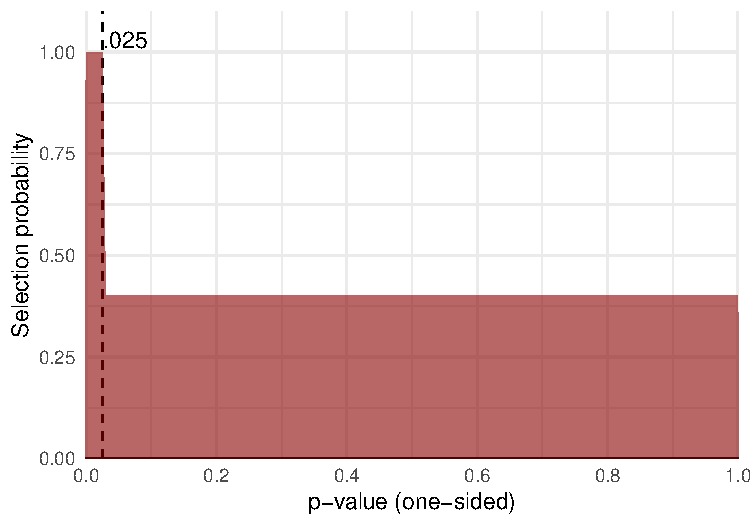
\includegraphics[width=0.49\linewidth]{step-function-selection-models-with-dependent-effects_files/figure-latex/step-functions-1} }\subfloat[Two-step selection with $\lambda_1 = 0.4, \lambda_2 = 0.2$\label{fig:step-functions-2}]{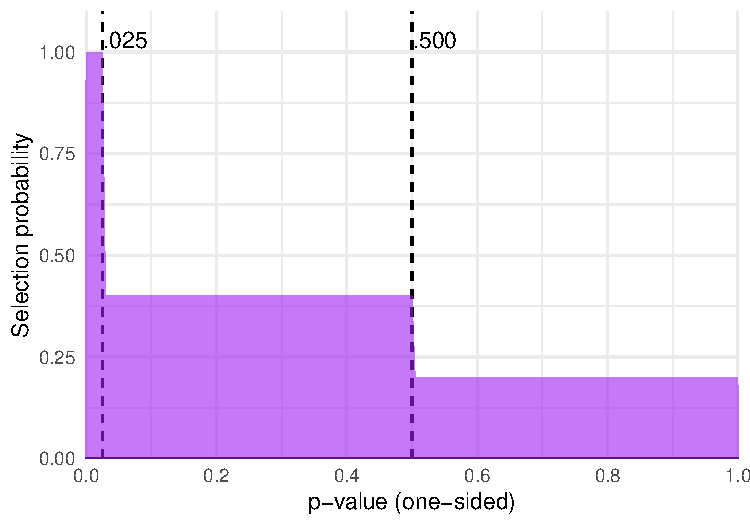
\includegraphics[width=0.49\linewidth]{step-function-selection-models-with-dependent-effects_files/figure-latex/step-functions-2} }\caption{Examples of step functions}\label{fig:step-functions}
\end{figure}

\subsection{Distribution of observed effect size estimates}\label{distribution-of-observed-effect-size-estimates}

Combining the assumptions of the evidence-generating process and the selection process leads to a model for an observed effect size estimate. The distribution of an observed effect size estimate is equivalent to the distribution of \(Y^*\) given that \(O = 1\).
The marginal density of an observed effect size estimate \(Y\) with standard error \(\sigma\) has the form
\begin{equation}
\label{eq:generic-selection}
f(Y = y | \sigma, \mathbf{x}) = \frac{1}{A(\mathbf{x}, \sigma; \boldsymbol\beta, \tau^2, \boldsymbol\lambda)} \times w\left(y, \sigma; \boldsymbol\lambda \right) \times \frac{1}{\sqrt{\tau^2 + \sigma^2}} \phi\left(\frac{y - \mathbf{x} \boldsymbol\beta}{\sqrt{\tau^2 + \sigma^2}}\right),
\end{equation}
where
\begin{equation}
\label{eq:generic-selection-A}
A(\mathbf{x}, \sigma; \boldsymbol\beta, \tau^2, \boldsymbol\lambda) =  \int_\mathbb{R} w\left(y, \sigma; \boldsymbol\lambda \right) \times  \frac{1}{\sqrt{\tau^2 + \sigma^2}}\phi\left(\frac{y - \mathbf{x}\boldsymbol\beta}{\sqrt{\tau^2 + \sigma^2}}\right) dy.
\end{equation}
If \(w(y, \sigma; \boldsymbol\lambda) = 1\), then there is no selective reporting, \(A(\mathbf{x}, \sigma; \boldsymbol\beta, \tau^2, \boldsymbol\lambda) = 1\), and the density reduces to the unweighted density of the evidence-generating process (i.e., the density of a random-effects meta-regression).
The \(A(\mathbf{x}, \sigma; \boldsymbol\beta, \tau^2, \boldsymbol\lambda)\) term can be computed using the closed-form expression
\begin{equation}
\label{eq:step-function-A}
A_{ij} = A(\mathbf{x}_{ij}, \sigma_{ij}; \boldsymbol\beta, \tau^2, \boldsymbol\lambda) = \sum_{h=0}^H \lambda_h B_{hij}
\end{equation}
where
\begin{equation}
\label{eq:step-function-Bhij}
B_{hij} = \Phi\left(c_{hij}\right) - \Phi\left(c_{h+1,ij}\right),
\end{equation}
and \(c_{hij} = \left(\sigma_{ij} \Phi^{-1}\left(1 - \alpha_h\right) - \mathbf{x}_{ij}\boldsymbol\beta\right) / \sqrt{\tau^2 + \sigma_{ij}^2}\) for \(h = 0,...,H\).\textsuperscript{26}

\subsection{Estimation Methods}\label{estimation-methods}

Past developments of selection models have focused either on maximum likelihood estimation under the assumption that all effect sizes are mutually independent\textsuperscript{25--27} or on sensitivity analysis methods that treat the selection model as known\textsuperscript{46,51}. We consider two estimation and inference strategies that build upon and generalize past approaches, including maximum composite marginal likelihood and an alternative based on re-weighting the Gaussian likelihood of the evidence-generating process.
With both approaches, we allow for incorporation of prior weights, which permits efficient calculation for a variety of bootstrapping techniques.
Thus, let \(a_{11},...,a_{J k_j}\) be an arbitrary set of prior weights assigned to each effect size estimate; in a typical, unweighted analysis, all weights will will be equal to \(a_{ij} = 1\).

\subsubsection{Maximum composite marginal likelihood}\label{maximum-composite-marginal-likelihood}

Composite marginal likelihood techniques involve working with the marginal distribution of each observed effect size estimate as if they were all mutually independent\textsuperscript{52--54}.
Thus, we assume that the observed effect size estimates were generated from Equation \eqref{eq:generic-selection}.
For purposes of estimation, we write the likelihoods using natural log transformations of the variance parameter and selection parameters, with \(\gamma = \log \tau^2\), \(\zeta_h = \log \lambda_h\), and \(\boldsymbol\zeta = \left[\zeta_1,...,\zeta_H\right]'\).
The log of the marginal likelihood contribution for effect size estimate \(i\) from study \(j\) is given by
\begin{align}
l^M_{ij}\left(\boldsymbol\beta, \gamma, \boldsymbol\zeta \right) &= \log f\left(Y = y_{ij} | \sigma_{ij}, \mathbf{x}_{ij}\right) \nonumber \\
&\propto \log w\left(y_{ij}, \sigma_{ij}; \boldsymbol\zeta \right) - \frac{1}{2} \frac{\left(y_{ij} - \mathbf{x}_{ij} \boldsymbol\beta\right)^2}{\exp(\gamma) + \sigma_{ij}^2} \nonumber\\
& \qquad \qquad  - \frac{1}{2}\log\left(\exp(\gamma) + \sigma_{ij}^2\right) - \log A\left(\mathbf{x}_{ij}, \sigma_{ij}; \boldsymbol\beta, \gamma, \boldsymbol\zeta \right). \label{eq:log-like-ij}
\end{align}
The weighted composite marginal log-likelihood across all \(J\) studies is then
\begin{equation}
\label{eq:marginal-likelihood}
l^M\left(\boldsymbol\beta, \gamma, \boldsymbol\zeta\right) = \sum_{j=1}^J \sum_{i=1}^{k_j} a_{ij} l^M_{ij}\left(\boldsymbol\beta, \gamma, \boldsymbol\zeta\right).
\end{equation}
The composite marginal likelihood (CML) estimators, denoted as \(\boldsymbol{\hat\beta}\), \(\hat\gamma\), and \(\boldsymbol{\hat\zeta}\), are obtained as the set of parameter values that maximize the composite likelihood for the observed data, as given in Equation (\ref{eq:marginal-likelihood}).

If the true parameter values are not at the extremes of their ranges, the CML estimator can also be defined as the solution of the weighted score equations,
\begin{equation}
\sum_{j=1}^J \mathbf{S}_{j}\left(\boldsymbol{\hat\beta}, \hat\gamma, \boldsymbol{\hat\zeta}\right) = \mathbf{0}
\end{equation}
where \(\mathbf{S}_j = \left(\mathbf{S}_{\boldsymbol\beta j}' \  S_{\gamma j} \ \mathbf{S}_{\boldsymbol\zeta j}'\right)'\) denotes the score vector from study \(j\), consisting of the derivatives of the likelihood contributions for each study with respect to the component parameters:
\begin{align}
\mathbf{S}_{\boldsymbol\beta j}\left(\boldsymbol{\beta}, \gamma, \boldsymbol{\zeta}\right) &= \sum_{i=1}^{k_j} a_{ij} \frac{\partial l^M_{ij}\left(\boldsymbol\beta, \gamma, \boldsymbol\zeta\right)}{\partial \boldsymbol\beta} \label{eq:score-M-beta} \\
S_{\gamma j}\left(\boldsymbol{\beta}, \gamma, \boldsymbol{\zeta}\right) &= \sum_{i=1}^{k_j} a_{ij} \frac{\partial l^M_{ij}\left(\boldsymbol\beta, \gamma, \boldsymbol\zeta\right)}{\partial \gamma} \label{eq:score-M-gamma} \\
\mathbf{S}_{\boldsymbol\zeta j}\left(\boldsymbol{\beta}, \gamma, \boldsymbol{\zeta}\right) &= \sum_{i=1}^{k_j} a_{ij} \frac{\partial l^M_{ij}\left(\boldsymbol\beta, \gamma, \boldsymbol\zeta\right)}{\partial \boldsymbol\zeta}. \label{eq:score-M-zeta} 
\end{align}
Online Appendix \ref{CML-derivatives} provides exact expressions for the score vectors of the step-function selection model.

Robust variance estimators, or sandwich estimators, are a commonly used technique for quantifying the uncertainty in CML estimators. Let \(\mathbf{H}\) denote the Hessian matrix of the composite log-likelihood,
\begin{equation}
\mathbf{H}(\boldsymbol\beta, \gamma, \boldsymbol\zeta) = \sum_{j=1}^J \frac{\partial \mathbf{S}_j(\boldsymbol\beta, \gamma, \boldsymbol\zeta)}{\partial \left(\boldsymbol\beta' \ \gamma \ \boldsymbol\zeta'\right)},
\end{equation}
exact expressions for which are given in Online Appendix \ref{CML-derivatives}.
Let \(\mathbf{\hat{S}}_j = \mathbf{S}_j(\boldsymbol{\hat\beta}, \hat\gamma, \boldsymbol{\hat\zeta})\) and \(\mathbf{\hat{H}} = \mathbf{H}(\boldsymbol{\hat\beta}, \hat\gamma, \boldsymbol{\hat\zeta})\) denote the score vectors and Hessian matrix evaluated at the maximum of the composite likelihood.
We then estimate the sampling variance of the CML estimator using a cluster-robust sandwich formula:
\begin{equation}
\label{eq:sandwich-variance}
\mathbf{V}^{CML} = \mathbf{\hat{H}}^{-1}\left(\sum_{j=1}^J \mathbf{\hat{S}}_j {\mathbf{\hat{S}}_j}'\right) \mathbf{\hat{H}}^{-1}.
\end{equation}
We construct confidence intervals for model parameters using \(\mathbf{V}^{CML}\) with Wald-type large sample approximations. For instance, the \((1 - 2\alpha)\)-level large-sample confidence interval for a meta-regression parameter \(\beta_g\) is constructed as
\[
\hat\beta_g \ \pm \ \Phi^{-1}(1 - \alpha) \times \sqrt{V^{CML}_{gg}},
\]
where \(V^{CML}_{gg}\) is the \(g^{th}\) diagonal entry of \(\mathbf{V}^{CML}\).

\subsubsection{Augmented, re-weighted Gaussian likelihood}\label{augmented-re-weighted-gaussian-likelihood}

Composite marginal likelihood is not the only possible basis for deriving estimators of selection model parameters.
In the framework of a sensitivity analysis for worst-case selection bias, Mathur and VanderWeele\textsuperscript{46} proposed using regular meta-analytic estimators for \(\boldsymbol\beta\), but with weights defined by the inverse probability of selection under a step-function selection model with a single step at \(\alpha_1 = .025\).
Because they were working in the context of sensitivity analysis, they assumed a maximum plausible degree of selection rather than estimating the parameters of a selection model, so that the weights were fixed and known quantities.
In contrast, here we will consider a more general model, possibly with multiple steps, using weights derived by estimating the selection model parameters.
We describe the estimators as augmented, re-weighted Gaussian likelihood (ARGL) estimators because the Gaussian likelihood of the evidence-generating process is re-weighted based on the selection process, with selection process parameters identified by augmenting the likelihood with an additional estimating equation.

Given the parameters of the selection process, we can calculate relative probabilities of selection for each effect size estimate, \(w_{ij} = w(y_{ij}, \sigma_{ij}; \boldsymbol\zeta)\). We use these selection probabilities to form weighted estimating equations for the evidence-generating process. Under the evidence-generation model, the marginal log-likelihood of effect size estimate \(i\) from study \(j\) is Gaussian, given by
\[
l^G_{ij}(\boldsymbol\beta, \gamma) \propto - \frac{1}{2}\frac{(y_{ij} - \mathbf{x}_{ij} \boldsymbol\beta)^2}{\exp(\gamma) + \sigma_{ij}^2} - \frac{1}{2}\log(\exp(\gamma) + \sigma_{ij}^2).
\]
Allowing for prior weights, the inverse selection-weighted Gaussian log-likelihood is therefore
\begin{equation}
l^G(\boldsymbol\beta, \gamma, \boldsymbol\zeta) = \sum_{j=1}^J \sum_{i=1}^{k_j} \frac{a_{ij}} {w_{ij}} \times l^G_{ij}(\boldsymbol\beta, \gamma).
\end{equation}
If the parameters of the selection process were known, we could find estimators for \(\boldsymbol\beta\) and \(\gamma\) by maximizing \(l^G(\boldsymbol\beta, \gamma, \boldsymbol\zeta)\) for a fixed value of \(\boldsymbol\zeta\).
Equivalently, we could find the estimators as the solutions to the weighted score equations
\begin{align}
\sum_{j=1}^J \mathbf{S}^G_{\boldsymbol\beta j} (\boldsymbol\beta, \gamma, \boldsymbol\zeta) &= 0 \label{eq:hybrid-score-beta} \\
\sum_{j=1}^J \mathbf{S}^G_{\gamma j} (\boldsymbol\beta, \gamma, \boldsymbol\zeta) &= 0, \label{eq:hybrid-score-gamma}
\end{align}
where the score contributions for study \(j\) are
\begin{align}
\mathbf{S}^G_{\boldsymbol\beta j} (\boldsymbol\beta, \gamma, \boldsymbol\zeta) &= \sum_{i=1}^{k_j} a_{ij} \times \mathbf{x}_{ij}' \frac{y_{ij} - \mathbf{x}_{ij} \boldsymbol\beta}{w_{ij} \left(\exp(\gamma) + \sigma_{ij}^2\right)} \\
\mathbf{S}^G_{\gamma j} (\boldsymbol\beta, \gamma, \boldsymbol\zeta) &= \sum_{i=1}^{k_j} a_{ij} \times \frac{\exp(\gamma)}{2 w_{ij}} \left(\frac{(y_{ij} -\mathbf{x}_{ij} \boldsymbol\beta)^2}{\left(\exp(\gamma) + \sigma_{ij}^2\right)^2} - \frac{1}{\exp(\gamma) + \sigma_{ij}^2}\right).
\end{align}
The question remains how to obtain an estimator for \(\boldsymbol\zeta\).

We propose to estimate \(\boldsymbol\zeta\) by augmenting the Gaussian log-likelihood with the marginal score equation with respect to \(\boldsymbol\zeta\).
Specifically, we define the ARGL estimators as the values that simultaneously solve Equations \eqref{eq:hybrid-score-beta} and \eqref{eq:hybrid-score-gamma} together with the estimating equation for \(\boldsymbol\zeta\) from the composite marginal likelihood approach.
With \(\mathbf{S}_{\boldsymbol\zeta j}\left(\boldsymbol{\beta}, \gamma, \boldsymbol{\zeta}\right)\) as given in Equation \eqref{eq:score-M-zeta}, the full set of estimating equations is
\begin{equation}
\label{eq:hybrid-score}
\mathbf{M}_j(\boldsymbol\beta, \gamma, \boldsymbol\zeta) = \left[\begin{array}{c} \mathbf{S}^G_{\boldsymbol\beta j}(\boldsymbol\beta, \gamma, \boldsymbol\zeta) \\ S^G_{\gamma j}(\boldsymbol\beta, \gamma, \boldsymbol\zeta) \\ \mathbf{S}_{\boldsymbol\zeta j}(\boldsymbol\beta, \gamma, \boldsymbol\zeta) \end{array}\right],
\end{equation}
based on which we define the ARGL estimator as the solution to the estimating equations
\begin{equation}
\label{eq:hybrid-total-score}
\sum_{j=1}^J \mathbf{M}_j(\boldsymbol\beta, \gamma, \boldsymbol\zeta) = \mathbf{0}.
\end{equation}
We will denote the ARGL parameter estimators as \(\boldsymbol{\tilde\beta}\), \(\tilde\gamma\), and \(\boldsymbol{\tilde\zeta}\).

We consider conducting inferences for the ARGL estimators using cluster-robust sandwich variance estimators that have the same form as (\ref{eq:sandwich-variance}).
Online Appendix \ref{ARGL-derivatives} provides further details.
We construct confidence intervals for model parameters using Wald-type large sample approximations, just as with the CML estimators.

\subsection{Bootstrap inference}\label{bootstrap-inference}

Sandwich estimators such as those in Equations \eqref{eq:sandwich-variance} require a large number of independent clusters (i.e., large \(J\)) to provide accurate assessments of uncertainty.
We consider alternative inference techniques based on bootstrapping, which might provide more accurate inference with a limited number of clusters.
Bootstrap techniques involve generating many new pseudo-samples of observations by randomly perturbing the original sample, then re-calculating an estimator using each pseudo-sample.
The distribution of the estimator across pseudo-samples is used as a proxy for the actual sampling distribution of the estimator, providing a basis for calculating standard errors and confidence intervals.

Many different bootstrap sampling schemes have been described that apply to different data structures and require different assumptions\textsuperscript{55}.
For data involving dependent observations, it is crucial that the process used to generate pseudo-samples accounts for the dependence structure.
Techniques that do so include the non-parametric clustered bootstrap, two-stage bootstrap\textsuperscript{56,57}, and fractional random weight bootstrap\textsuperscript{58}.
Here, we focus on the two-stage bootstrap; details about other bootstrap techniques can be found in Online Appendix \ref{bootstrap-details}.

In the two-stage bootstrap, each pseudo-sample is generated by randomly drawing \(J\) clusters of observations with replacement from the original sample and then randomly re-sampling observations with replacement from each selected cluster.
This process amounts to simulating set of weights. Let \(a_j^{(b)}\) be a first-stage weight for cluster \(j\) and \(a_{ij}^{(b)}\) be the weight assigned to observation \(i\) in cluster \(j\) for pseudo-sample \(b\).
The two-stage bootstrap is equivalent to first drawing \(a_1^{(b)},...,a_J^{(b)}\) from a multinomial distribution with \(J\) trials and equal probability on each of \(J\) categories, then drawing \(a_{1j}^{(b)},...,a_{k_j j}^{(b)}\) from a multinomial distribution with \(a_j^{(b)} \times k_j\) trials and equal probability on each of \(k_j\) categories, for \(j = 1,...,J\).

For constructing confidence intervals, bootstrapping entails generating a total of \(B\) pseudo-samples, where \(B\) is a large number such as 1999, and re-calculating the estimator for each pseudo-sample.
There are several methods for constructing confidence intervals from a bootstrap distribution.
We consider four standard methods\textsuperscript{55}, including the percentile CI, basic CI, studentized CI, and the bias-corrected-and-accelerated CI proposed by\textsuperscript{59}.
Online Appendix \ref{bootstrap-details} provides further details about the bootstrap CI calculations.

\section{Empirical Example}\label{empirical-example}

To demonstrate the proposed modeling strategy and examine potential differences between CML and ARGL estimation methods, we re-analyzed a subset of data from a meta-analysis on the ego depletion effect\textsuperscript{60}.
Ego depletion refers to the theory that an individual's ability to exercise self-control diminishes with repeated exertion\textsuperscript{61}.
Carter and colleagues\textsuperscript{60} argued that the apparent strength of ego-depletion effects may be overstated due to selective reporting.
Their review included a variety of self-control manipulation tasks as well as a range of outcomes.
Some primary studies reported effects for multiple outcome tasks, leading to dependent effects.
Effect sizes were measured as standardized mean differences, defined so that positive effects correspond to depletion of self-control, consistent with the theory of ego depletion.

To mitigate possible effects of selective reporting, the original review included many unpublished studies\textsuperscript{60}.
For illustrative purposes, we re-analyzed the findings from the subset of published studies only; we also excluded a single outlying effect size estimate that was greater than 2. This analytic sample includes 66 effect size estimates from 45 distinct studies.
We conducted the analyses using R Version 4.4.3\textsuperscript{62}.

If selective reporting were not a concern, a correlated-and-hierarchical effects (CHE) model would be one way to summarize the distribution of ego depletion effects.\textsuperscript{42}
Based on a CHE model, the overall average effect estimate was 0.46, 95\% CI {[}0.34, 0.59{]}.
Alternately, one could apply a CHE model with inverse sampling covariance weighting (CHE-ISCW), which places relatively more weight on larger studies (those with smaller sampling variances) and thus is less biased by selective reporting.\textsuperscript{49}
Applying CHE-ISCW reduces the overall effect estimate to 0.39, 95\% CI {[}0.24, 0.54{]}.
As a further point of comparison, we estimated the overall average effect using the PET/PEESE regression adjustment\textsuperscript{20}, clustering the standard errors by study. This yielded an overall average effect of -0.09, 95\% CI {[}-0.76, 0.58{]}. The CHE and CHE-ISCW estimates are both positive, significant, and similar in magnitude. The PET-PEESE estimate is negative and much smaller than the CHE and CHE-ISCW estimates, indicating a pattern of small study effects.

We used the \texttt{selection\_model()} function from the \texttt{metaselection} package to fit single-step and two-step selection models\textsuperscript{63}.
The single-step model used a threshold at \(\alpha_1 = 0.025\); the two-step model used thresholds at \(\alpha_1 = 0.025\) and \(\alpha_2 = 0.5\).
For comparison purposes, we estimated model parameters using both CML and ARGL and computed cluster-robust and percentile bootstrap confidence intervals.
For bootstrapping, we used two-stage cluster bootstrap re-sampling with 1999 replicates.

Table \ref{tab:empirical} presents the parameter estimates from the one-step and two-step selection models.
The estimated selection parameters are similar across the one- and two-step models and across both estimators, all indicating that non-significant or negative effect size estimates were less likely to be reported than statistically significant, affirmative ones.
The one-step and two-step selection model estimates of average effect size are positive but substantially smaller than the CHE-ISCW estimates, ranging from 0.23 to 0.27 depending on the model specification and estimation method.
In contrast to the PET/PEESE estimate, the selection model estimates using CML are positive and statistically distinct from zero.
Thus, an analyst would reach different conclusions about overall average effect size depending on whether they use an unadjusted model, a step-function model, or the PET/PEESE adjustment.

\begin{table}[tb]
\centering
\caption{\label{tab:empirical}Single-step and two-step selection model parameter estimates fit to ego depletion effects data from Carter et al. (2015)}
\centering
\resizebox{\ifdim\width>\linewidth\linewidth\else\width\fi}{!}{
\begin{threeparttable}
\begin{tabular}[t]{l>{\raggedright\arraybackslash}p{5.5em}>{\raggedright\arraybackslash}p{5.5em}>{\raggedright\arraybackslash}p{5.5em}>{\raggedright\arraybackslash}p{5.5em}>{\raggedright\arraybackslash}p{5.5em}>{\raggedright\arraybackslash}p{5.5em}}
\toprule
\multicolumn{1}{c}{ } & \multicolumn{3}{c}{CML estimator} & \multicolumn{3}{c}{ARGL estimator} \\
\cmidrule(l{3pt}r{3pt}){2-4} \cmidrule(l{3pt}r{3pt}){5-7}
Parameter & Estimate (SE) & Cluster-Robust CI & Percentile Bootstrap CI & Estimate (SE) & Cluster-Robust CI & Percentile Bootstrap CI\\
\midrule
\addlinespace[0.3em]
\multicolumn{7}{l}{\textbf{One-step}}\\
\hspace{1em}$\beta$ & 0.25 (0.09) & {}[ 0.07,      0.44] & {}[ 0.05, 0.47] & 0.27 (0.07) & {}[ 0.14,      0.41] & {}[ 0.11, 0.47]\\
\hspace{1em}$\tau^2$ & 0.11 (0.04) & {}[ 0.06,      0.20] & {}[ 0.02, 0.19] & 0.11 (0.04) & {}[ 0.06,      0.21] & {}[ 0.01, 0.21]\\
\hspace{1em}$\lambda_1$ & 0.27 (0.14) & {}[ 0.10,      0.75] & {}[ 0.07, 0.87] & 0.30 (0.10) & {}[ 0.16,      0.56] & {}[ 0.05, 1.20]\\
\addlinespace[0.3em]
\multicolumn{7}{l}{\textbf{Two-step}}\\
\hspace{1em}$\beta$ & 0.23 (0.11) & {}[ 0.02,      0.44] & {}[-0.01, 0.48] & 0.25 (1.45) & {}[-2.59,      3.10] & {}[-0.05, 0.54]\\
\hspace{1em}$\tau^2$ & 0.11 (0.04) & {}[ 0.06,      0.21] & {}[ 0.03, 0.19] & 0.12 (0.33) & {}[ 0.00,     32.00] & {}[ 0.00, 0.20]\\
\hspace{1em}$\lambda_1$ & 0.27 (0.14) & {}[ 0.10,      0.74] & {}[ 0.07, 0.86] & 0.29 (1.65) & {}[ 0.00,>100] & {}[ 0.05, 1.28]\\
\hspace{1em}$\lambda_2$ & 0.22 (0.16) & {}[ 0.06,      0.90] & {}[ 0.04, 1.18] & 0.26 (2.17) & {}[ 0.00,>100] & {}[ 0.01, 3.14]\\
\bottomrule
\end{tabular}
\begin{tablenotes}
\item \textit{Note: } 
\item ARGL = augmented, reweighted gaussian likelihood; CML = composite maximum likelihood; CI = confidence interval; SE = standard error.
\end{tablenotes}
\end{threeparttable}}
\end{table}

The estimates in Table \ref{tab:empirical} point towards some potential differences between estimation methods.
Generally, the CML and ARGL parameter estimates are similar in magnitude, but the confidence intervals based on the CML estimator are narrower than those for the ARGL estimator.
For the CML estimator, the bootstrap CIs are similar or slightly wider than the cluster-robust CIs.
These patterns suggest that there could be differences in the performance of the estimators, as well as differences in performance between the step-function estimators and alternative adjustment methods such as PET/PEESE.
However, these results are based on a single empirical dataset where the true data-generating process is unknown.
To draw firmer conclusion about these methods, we conducted simulations to evaluate their performance characteristics across a range of conditions.

\section{Simulation Methods}\label{simulation-methods}

We conducted Monte Carlo simulation studies to examine the performance
of the CML and ARGL estimators for a step-function selection model with a single step, under a wide range of conditions where primary studies contribute multiple, statistically dependent effect size estimates.
We compare the performance of these novel estimators to two available alternatives: a summary meta-analysis that addresses the dependency structure but does not correct for selective reporting and the PET-PEESE adjustment\textsuperscript{20}.
We evaluated the estimators in terms of convergence rates, bias, accuracy, and confidence interval coverage for recovering the average effect size prior to selective reporting.
To limit the computational burden, we evaluated the performance of bootstrap confidence intervals only for a subset of the conditions.

We ran the simulation in R Version 4.4.1\textsuperscript{62} using the high-throughput computing cluster at the University of Wisconsin - Madison\textsuperscript{64}.
The simulation code made use of several R packages, including \texttt{metafor}\textsuperscript{65}, \texttt{clubSandwich}\textsuperscript{66}, \texttt{simhelpers}\textsuperscript{67}, \texttt{optimx}\textsuperscript{68}, \texttt{nleqslv}\textsuperscript{69}, and \texttt{tidyverse}\textsuperscript{70}.

\subsection{Data generation}\label{data-generation}

We simulated meta-analyses based on a CHE working model, with individual effect size estimates selected
for inclusion based on the step-function selection model with a single step at \(\alpha_1 = .025\).
For each replication, we generated a total of \(J^*\) studies with a two-group comparison
design, where study \(j\) had an effective sample size of \(N_j\) and contributed \(k_j^* \geq 1\) effect size estimates prior to selective reporting.
To generate each meta-analytic dataset, we sampled effective sample sizes\footnote{For studies that involved cluster-level treatment assignment, we computed effective sample sizes that account for the dependence of observations nested within clusters rather than using the raw participant-level sample sizes.} and numbers of effect sizes per study from an empirical distribution based on the What Works Clearinghouse database.
The total effective sample size per study was divided equally into two groups, treatment and control.
We then generated \(r_j\), an outcome correlation for study \(j\), by drawing from a beta distribution with mean \(\rho\) and standard deviation 0.05.
We assumed constant correlation between pairs of outcomes within a study but allowed the correlation to vary from study to study.

We then simulated raw outcomes for each primary study included in the
meta-analytic dataset. To do so, we first generated an average effect
size per study, \(\delta_j\), from a normal distribution with mean \(\mu\) and variance
of \(\tau^2\). Given \(\delta_j\), we generated \(k_j^*\) effect size parameters per study, \(\boldsymbol\delta_j = \left(\delta_{1j},...,\delta_{k_j^* j}\right)'\), from a normal distribution with mean of \(\delta_j\) and
variance of \(\omega^2\).
For each of the \(N_j / 2\) participants in the treatment and control groups, we then simulated vectors of multivariate normal outcomes as \(\mathbf{Y}_{hj}^T \sim N(\boldsymbol\delta_j, \boldsymbol\Psi_j)\) and \(\mathbf{Y}_{hj}^C \sim N(\mathbf{0}, \boldsymbol\Psi_j)\), where \(\mathbf{Y}_{hj}^T\) and \(\mathbf{Y}_{hj}^C\) are
\(k_j^* \times 1\) vectors of outcomes for participant \(h\) in study \(j\) in the treatment and control group, respectively, and \(\boldsymbol\Psi_j\) is the covariance matrix for outcomes in study \(j\), with diagonal elements equal to 1 and off-diagonal elements equal to \(r_j\).
From the raw outcome data, we calculated standardized mean
differences using Hedges's \(g\) bias correction for each of the correlated outcomes, yielding effect size estimates \(y^*_{ij}\) for \(i=1,...,k_j^*\) and \(j = 1,...,J^*\).
We calculated the sampling variances using conventional formulas\textsuperscript{71} and computed one-sided \(p\)-values based on two-sample \(t\)-tests for the null of \(H_0: \delta_{ij} \leq 0\).

After simulating results for study \(j\), we applied a step-function selection
model to the individual effect size estimates, with a one-sided selection
threshold at \(\alpha = 0.025\). Specifically, we let result \((y^*_{ij},
\sigma_{ij}^*, p_{ij}^*)\) be included in the observed dataset with probability
1 if \(p_{ij}^*\) was less than 0.025 and with probability \(0 < \lambda_1 \leq 1\) if \(p_{ij}^* \ge 0.025\).
We repeated the process of generating studies until the database included a total of \(J\) studies with at least one observed result, where observed study \(j\) includes \(k_j\) effect size estimates for \(1 \leq k_j \leq k_j^*\).

\subsection{Estimation methods}\label{estimation-methods-1}

We estimated step-function selection models with a single step at \(\alpha_1 = 0.025\), so that the assumed marginal selection process is consistent with the actual selective reporting process used to generate meta-analytic datasets.
We estimated CML and ARGL estimators and calculated cluster-robust confidence intervals as described in Section \ref{estimation-methods}.
For a subset of simulation conditions, we also examined percentile, basic, studentized, and bias-corrected-and-accelerated bootstrap confidence intervals based on the non-parametric two-stage bootstrap, clustered bootstrap, and fractional random weight bootstrap as described in Online Appendix \ref{bootstrap-details}.
To maintain computational feasibility, we used \(B = 399\) bootstrap replications of each estimator.

We compared the performance of the step-function CML and ARGL estimators to two alternative methods.
First, we estimated a summary meta-analysis model without any correction for selective reporting, using a method that accounts for effect size dependency.
Specifically, we used the CHE working model with inverse sampling-covariance weights (CHE-ISCW)\textsuperscript{49}.
We estimated the variance components using restricted maximum likelihood and assumed a sampling correlation of 0.8 for all pairs of effect size estimates from the same study, which leads to a degree of mis-specification when the average correlation used in the data-generating process differs from 0.80.
Second, we implemented a variation of the PET/PEESE estimator originally proposed by\textsuperscript{20}, adapted to accommodate dependent effect sizes.
Following convention, we combined the estimators by using PEESE if the PET estimator is statistically distinct from zero at an \(\alpha\)-level of 0.10, and otherwise using PET.\textsuperscript{20}
For the PET/PEESE and CHE-ISCW estimators, we calculated confidence intervals using cluster-robust variance estimation with the CR2 small-sample correction and Satterthwaite degrees of freedom\textsuperscript{49}.

\subsection{Experimental design}\label{experimental-design}

Table \ref{tab:sim-design} summarizes the experimental design for this study.
Manipulated parameters included overall average standardized mean difference
(\(\mu\)), between-study heterogeneity (\(\tau\)), within-study heterogeneity ratio
(\(\omega^2 / \tau^2\)), average correlation between outcomes (\(\rho\)),
probability of selection for non-affirmative results (\(\lambda_1\)), number of observed studies (\(J\)), and primary study sample size.
We examined values for the overall average SMD (\(\mu\)) ranging from 0.0 to 0.80, which covers the range of effects observed in a review of 747 randomized control trials of education interventions\textsuperscript{72}.
We used values of \(\tau\) ranging from 0.05 (a very small degree of heterogeneity) to 0.45 (a large degree of heterogeneity).
We specified the degree of within-study heterogeneity in relative terms, by setting the ratio of \(\omega^2\) to between-study heterogeneity \(\tau^2\) at either 0 (i.e., no within-study heterogeneity) or 0.5.
For the average correlation between outcomes from the same study, we examined the values of 0.40 or 0.80. The default value of the average
correlation in software packages that implement RVE is 0.80.
Thus, in conditions where \(\rho\) is 0.80, the working model is approximately correctly specified.
We included conditions where \(\rho = 0.4\) to examine performance when the working model is not correctly specified.

\begin{table}[tb]
\centering
\caption{\label{tab:sim-design}Parameter values examined in the simulation study}
\centering
\begin{tabular}[t]{>{\raggedright\arraybackslash}p{2.5in}ll}
\toprule
Parameter & Full Simulation & Bootstrap Simulation\\
\midrule
Overall average SMD ($\mu$) & 0.0, 0.2, 0.4, 0.8 & 0.0, 0.2, 0.4, 0.8\\
Between-study heterogeneity ($\tau$) & 0.05, 0.15, 0.30, 0.45 & 0.15, 0.45\\
Heterogeneity ratio ($\omega^2 / \tau^2$) & 0.0, 0.5 & 0.0, 0.5\\
Average correlation between outcomes ($\rho$) & 0.40, 0.80 & 0.80\\
Probability of selection for non-affirmative effects ($\lambda_1$) & 0.02, 0.05, 0.10, 0.20, 0.50, 1.0 & 0.05, 0.20, 1.0\\
\addlinespace
Number of observed studies ($J$) & 15, 30, 60, 90, 120 & 15, 30, 60\\
Primary study sample size & Typical, Small & Typical, Small\\
\bottomrule
\end{tabular}
\end{table}

We examined a wide range of values for the probability of selection for non-affirmative effect sizes, ranging from no selective reporting (\(\lambda_1 = 1\)) to very severe selective reporting \((\lambda_1 = 0.02)\).
We also examined a wide range of conditions for the number of primary studies included in the meta-analysis, ranging from relatively small databases of \(J = 15\) to very large databases with \(J = 120\) studies.
We chose these values to cover the conditions found in real meta-analyses of education and psychology research\textsuperscript{36}.

Lastly, we investigated the primary study sample size.
For the typical primary study sample sizes, we used the empirical distribution of sample sizes in the What Works Clearinghouse database of findings from educational intervention studies.
The sample sizes in the database ranged from 37 to 2,295 with a median of 211.
The number of effect sizes ranged from 1 to 48 with a median of 3.
To explore the influence of the effective sample size distribution, we also ran conditions in which we divided the sample
sizes from the What Works Clearinghouse database by three to represent primary studies with smaller sample sizes,
such as those used in psychology laboratory studies.

Parameters were fully crossed for a total of \(4 \times 4 \times 2 \times 2 \times 6 \times 5 \times 2 = 3,840\) conditions in the full simulation study.
Due to the computational demands of bootstrapping, we focused the bootstrap simulations on conditions with fewer studies per meta-analysis, for which we expected large-sample cluster-robust CIs to be relatively less effective.
We also reduced the number of parameter values for factors where we did
not observe much variation in results in the full simulation
(e.g., excluding \(\tau = 0.30\)).
This resulted in \(4 \times 2 \times 2 \times 1 \times 3 \times 3 \times 2 = 288\) conditions for the bootstrap simulations.
For each condition, we generated 2,000 replications.

\subsection{Performance criteria}\label{performance-criteria}

We evaluated the performance of these methods in terms of convergence rates, bias,
scaled root mean-squared error (RMSE), and 95\% confidence interval coverage for the overall average effect size \(\mu\).
Because we expected that RMSE would decrease proportionally with the square-root of the number of studies, we scaled the RMSE of each estimator by \(\sqrt{J}\) to reduce variation across the number of studies included in each meta-analysis.
Because the sampling distribution of the CML and ARGL estimators sometimes included extreme outlying values, we calculated bias and scaled RMSE after winsorizing the distribution.
Specifically, we defined a lower fence of 2.5 times the inter-quartile range below the 25th percentile and an upper fence of 2.5 times the inter-quartile range above the 75th percentile.
Estimates falling below the lower fence or above the upper fence were set to the corresponding fence values.

For confidence intervals based on cluster-robust variance estimation, we calculated coverage rates as the proportion of simulated intervals that included the true parameter.
For bootstrap confidence intervals, estimation of coverage rates is complicated by the fact that coverage is affected by the number of bootstrap replications.
To mitigate computational demand, we used few bootstraps per replication than recommended for analysis of real data.
To estimate coverage rates for confidence intervals as would be used in practice, we used an extrapolation technique\textsuperscript{73}.
For each replication, we computed bootstrap confidence intervals not only for \(B = 399\), but also for \(B = 49\), 99, 199, and 299 bootstraps, randomly selected without replacement.
We computed coverage rates separately for each value of \(B\), fit a linear regression of the coverage rate on \(1 / B\), and then used this regression to predict the coverage rate of confidence intervals based on \(B = 1999\) bootstraps.

\section{Simulation Results}\label{simulation-results}

We organize our presentation of simulation results by first considering the properties of point estimators for the average effect size.
For this parameter, we compare the bias and accuracy of the CML and ARGL estimators to that of the CHE-ISCW estimator and the PET/PEESE estimator.
We then examine the calibration of cluster-robust and bootstrap confidence intervals based on the CML and ARGL estimators.
Online Appendix \ref{gamma-simulation-results} includes additional results regarding the bias and accuracy of estimators of the marginal variance of the effect size distribution; Online Appendix \ref{zeta-simulation-results} has additional results on the performance of the CML and ARGL estimators for the selection parameter.

\subsection{Convergence}\label{convergence}

The CHE-ISCW and PET/PEESE estimators produced results for every replication in every condition.
The CML and ARGL estimators for the step-function selection model had very high convergence rates across most conditions, although the CML estimator did exhibit rates of convergence below 99\% under conditions with the lowest degree of heterogeneity \(\tau = 0.05\), with the lowest convergence rate of 94.40\%.
For the ARGL estimator, convergence was above 99.80\% across all conditions.
Supplementary Figure \ref{fig:convergence-rates} depicts the range of convergence rates of the CML and ARGL estimators.
We evaluated the performance characteristics of each estimator across the replications where it converged.

\subsection{Bias}\label{bias}

\begin{sidewaysfigure}
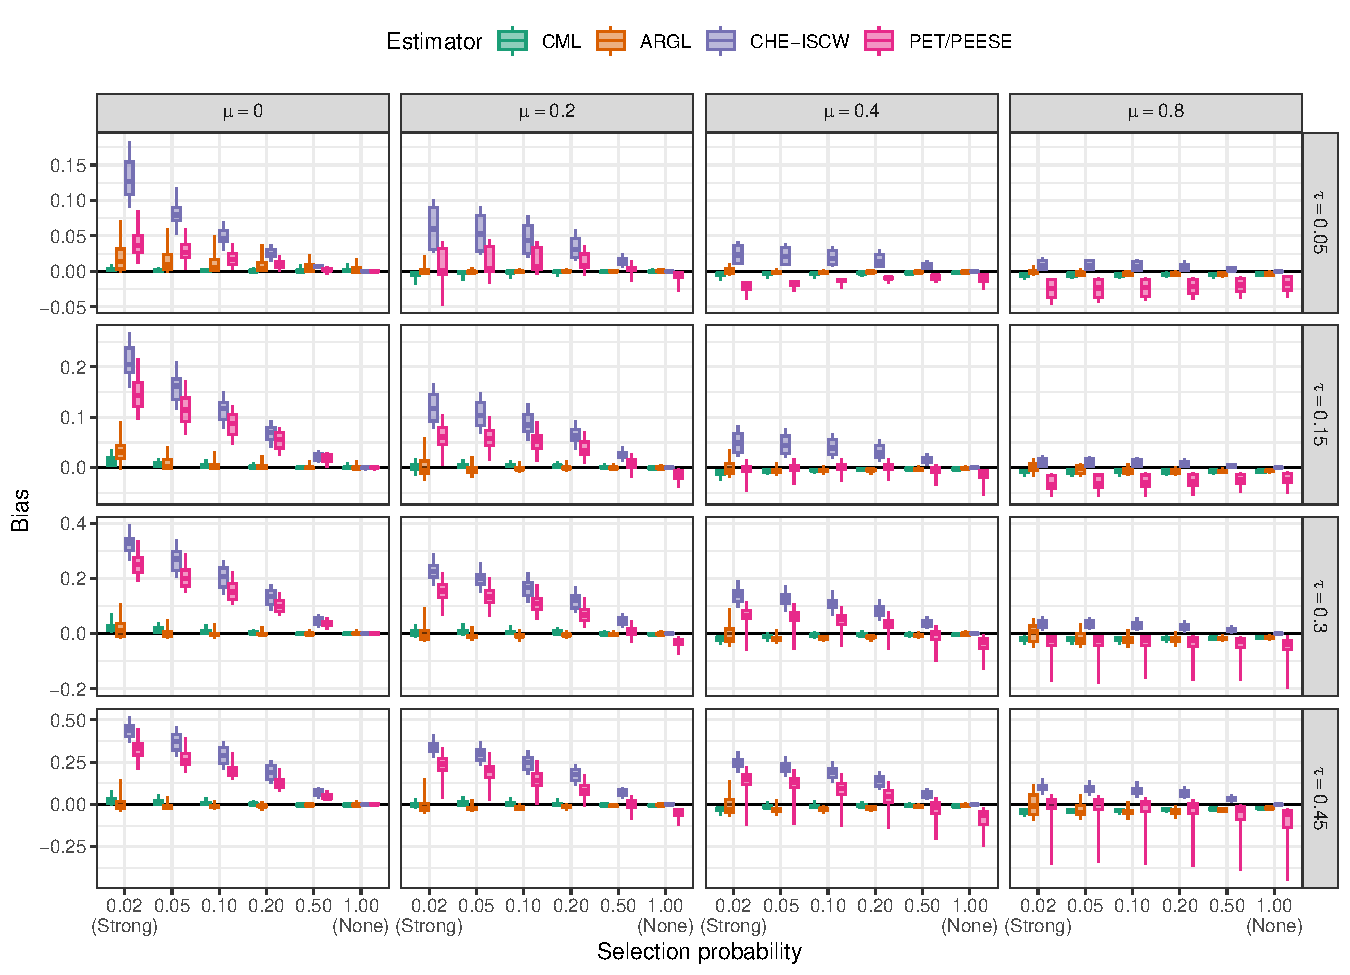
\includegraphics{step-function-selection-models-with-dependent-effects_files/figure-latex/mu-bias-1} \caption{Bias for estimators of average effect size by selection probability, average SMD, and between-study heterogeneity}\label{fig:mu-bias}
\end{sidewaysfigure}

Figure \ref{fig:mu-bias} depicts the bias (represented on the vertical axis of each plot) of each estimator of average effect size as a function of the strength of selective reporting (horizontal axis), average effect size parameter (varying by grid column), and between-study heterogeneity (\(\tau\), varying by grid row).
The box plot for each estimator depicts variation in bias over the remaining factors in the simulation design, which include the heterogeneity ratio, correlation between effect size estimates, number of observed studies, and primary study sample size distribution.
Note that the range of the vertical axis differs by grid row because the bias of some estimators is strongly influenced by the degree of heterogeneity.

The CML estimator has negligible or small bias across all conditions.
Its largest bias is 0.08, occurring when selective reporting is very strong, average effect size is zero, and heterogeneity is large.
The small bias of the CML estimator is stable across varying degrees of outcome correlation, within-study heterogeneity, number of observed studies, and primary study sample size.
Similar to the CML estimator, the ARGL estimator also has negligible or small bias across most conditions, although its bias increases when average effect is zero and selection is very strong.

In contrast to the estimators based on the marginal selection model, the CHE-iSCW and PET/PEESE estimators are systematically biased under many conditions.
The CHE-ISCW estimator, which does not directly adjust for selective reporting, is systematically biased under conditions with non-null selection.
When average effect size is large \((\mu = 0.8)\), its bias remains quite small even when selective reporting is very strong.
However, the bias of CHE-ISCW grows stronger when selection is more extreme, when average effect size is smaller, and when heterogeneity is larger; its bias exceeds 0.50 when \(\mu = 0.0\), \(\tau = 0.45\), and \(\lambda_1 = 0.02\).
Although the PET/PEESE estimator uses a regression adjustment to account for possible selective reporting, it too becomes severely biased when selective reporting is strong.
For smaller values of average effect size \((\mu \leq 0.2)\), the bias of PET/PEESE tracks the bias of the CHE-ISCW estimator but is somewhat less pronounced. Its bias grows larger (and closer to that of CHE-ISCW) for smaller values of average effect size and higher levels of heterogeneity.
For larger values of average effect size \((\mu = 0.8)\), the PET/PEESE estimator systematically under-estimates the average effect size---especially at high levels of heterogeneity.

\subsection{Scaled RMSE}\label{scaled-rmse}

\begin{sidewaysfigure}
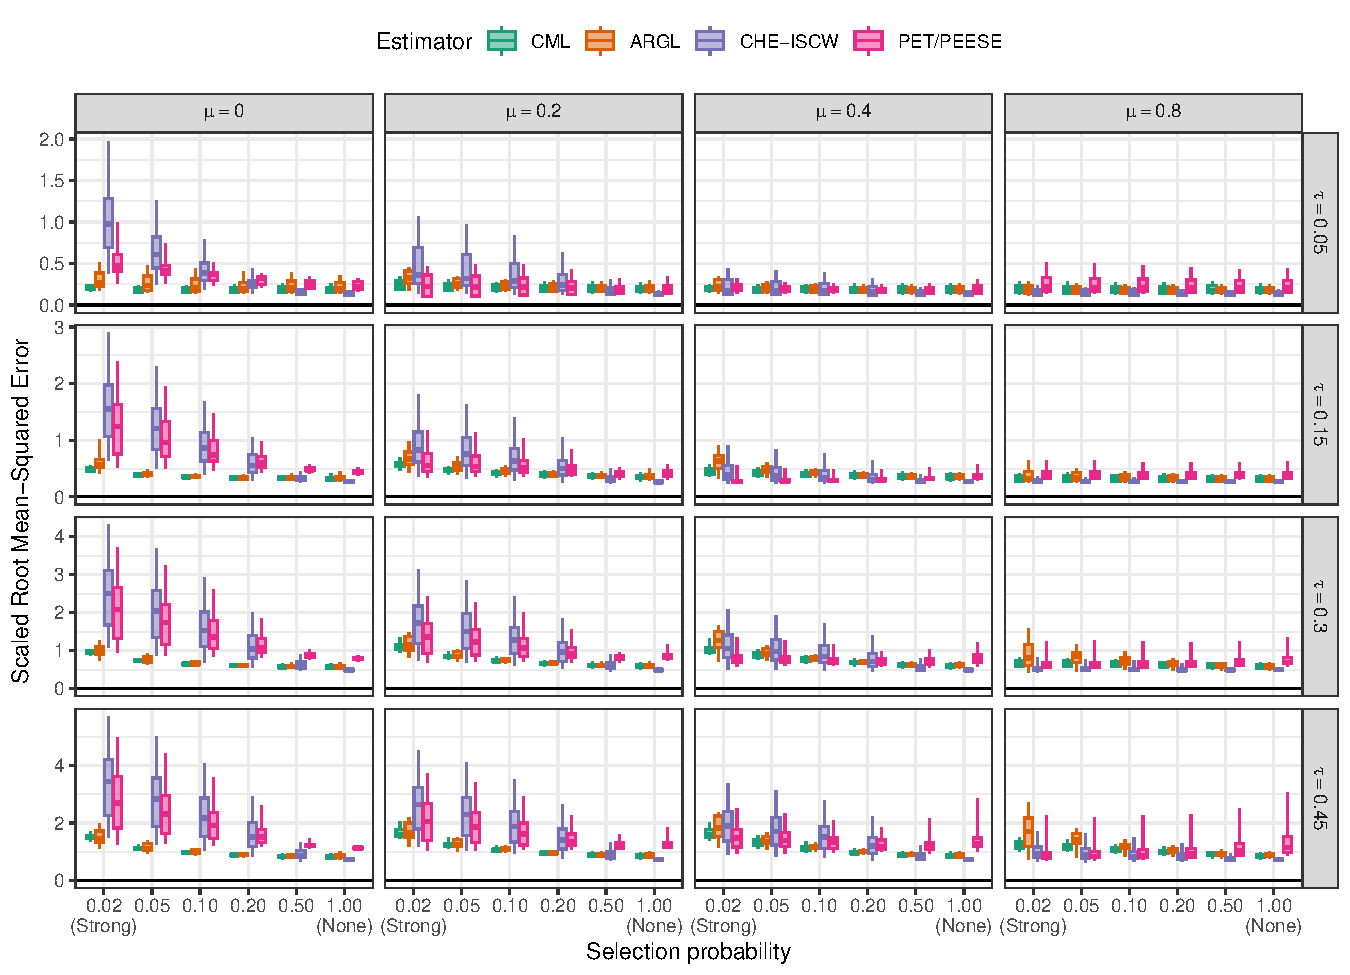
\includegraphics{step-function-selection-models-with-dependent-effects_files/figure-latex/mu-rmse-1} \caption{Scaled root mean-squared error for estimators of average effect size by selection probability, average SMD, and between-study heterogeneity}\label{fig:mu-rmse}
\end{sidewaysfigure}

Scaled RMSE combines both bias and variability into an overall measure of inaccuracy.
Figure \ref{fig:mu-rmse} depicts the scaled RMSE of each estimator of average effect size; it is constructed in the same way as Figure \ref{fig:mu-bias}.
Figures \ref{fig:rmse-ARGL-CML} through \ref{fig:rmse-PET-ARGL} in Online Appendix \ref{mu-simulation-results} provide greater detail about the relative accuracy of the four methods by plotting the ratio of RMSEs for each pair of methods.
These figures illustrate several findings.

First, across most data-generating conditions, the ARGL estimator has higher RMSE than the CML estimator. As evident in Figure \ref{fig:rmse-ARGL-CML}, the RMSE ratio comparing ARGL to CML is greater than one across most conditions examined.
The ARGL estimator has lower RMSE only under conditions of very high heterogeneity and in databases with few studies.
Thus, the CML estimator will typically be preferable to the ARGL estimator.

Second, considering both the selection model estimators and comparison methods, no single method achieves the lowest RMSE uniformly across all conditions examined.
Instead, all methods face bias-variance trade-offs.
Under conditions with small or moderate average effect size and moderate or strong selection, the selection model estimators generally have lower RMSE than the CHE-ISCW and PET/PEESE estimators.
The CML estimator has lower RMSE than CHE-ISCW under most conditions where selective reporting creates meaningful bias---specifically, for \(\lambda_1 <= 0.2\) and \(\mu \leq 0.2\) (Figure \ref{fig:rmse-CHE-CML}).
The relative accuracy of the ARGL estimator versus CHE-ISCW follows a similar pattern (Figure \ref{fig:rmse-CHE-ARGL}).

Third, the CML estimator also has lower RMSE than PET/PEESE under conditions where selective reporting creates meaningful bias, although it is not uniformly more accurate than PET/PEESE (Figure \ref{fig:rmse-PET-CML}).
Rather, PET/PEESE is more accurate under \emph{some} conditions involving moderate or large effect size \((\mu \geq 0.4)\) and varying degrees of between-study heterogeneity,
which correspond to conditions where the bias of PET/PEESE is small.
The relative accuracy is difficult to characterize generally because it follows a non-linear pattern involving interactions among the data-generating parameters.
The pattern of relative accuracy is very similar for the ARGL estimator (Figure \ref{fig:rmse-PET-ARGL}).

\subsection{Confidence Interval Coverage}\label{confidence-interval-coverage}

Figure \ref{fig:comparison-coverage} shows the coverage rates of 95\% CIs based on large-sample cluster-robust variance estimators for the CHE-ISCW, PET/PEESE, CML, and ARGL estimators.\footnote{To provide greater detail, the vertical axis of Figure \ref{fig:comparison-coverage} is limited to the range {[}0.5, 1.0{]}, and coverage rates of the CHE-ISCW and PET/PEESE intervals are not depicted when they fall below 0.5. Supplementary Figure \ref{fig:comparison-coverage-full} depicts the full range of coverage rates.}
Coverage rates are below the nominal rate of 0.95 for all methods across most conditions.
The CML and ARGL estimators based on the step-function selection model have higher coverage rates than the comparison methods under many conditions, particularly in conditions with higher between-study heterogeneity,\\
Intervals based on the CML and ARGL estimators have coverage levels that improve towards 0.95 as the number of studies increases, but are often still unacceptably low even when \(J\) is 90 or greater.
In contrast, intervals based on CHE-ISCW and PET/PEESE are often wildly mis-calibrated.
Under conditions where CHE-ISCW and PET/PEESE are biased by selective reporting, their confidence intervals do not center on the true parameter. Consequently, as the number of studies increases, the standard error of the estimators decreases (as does the width of confidence intervals) and their coverage rates degrade towards zero.

\begin{sidewaysfigure}
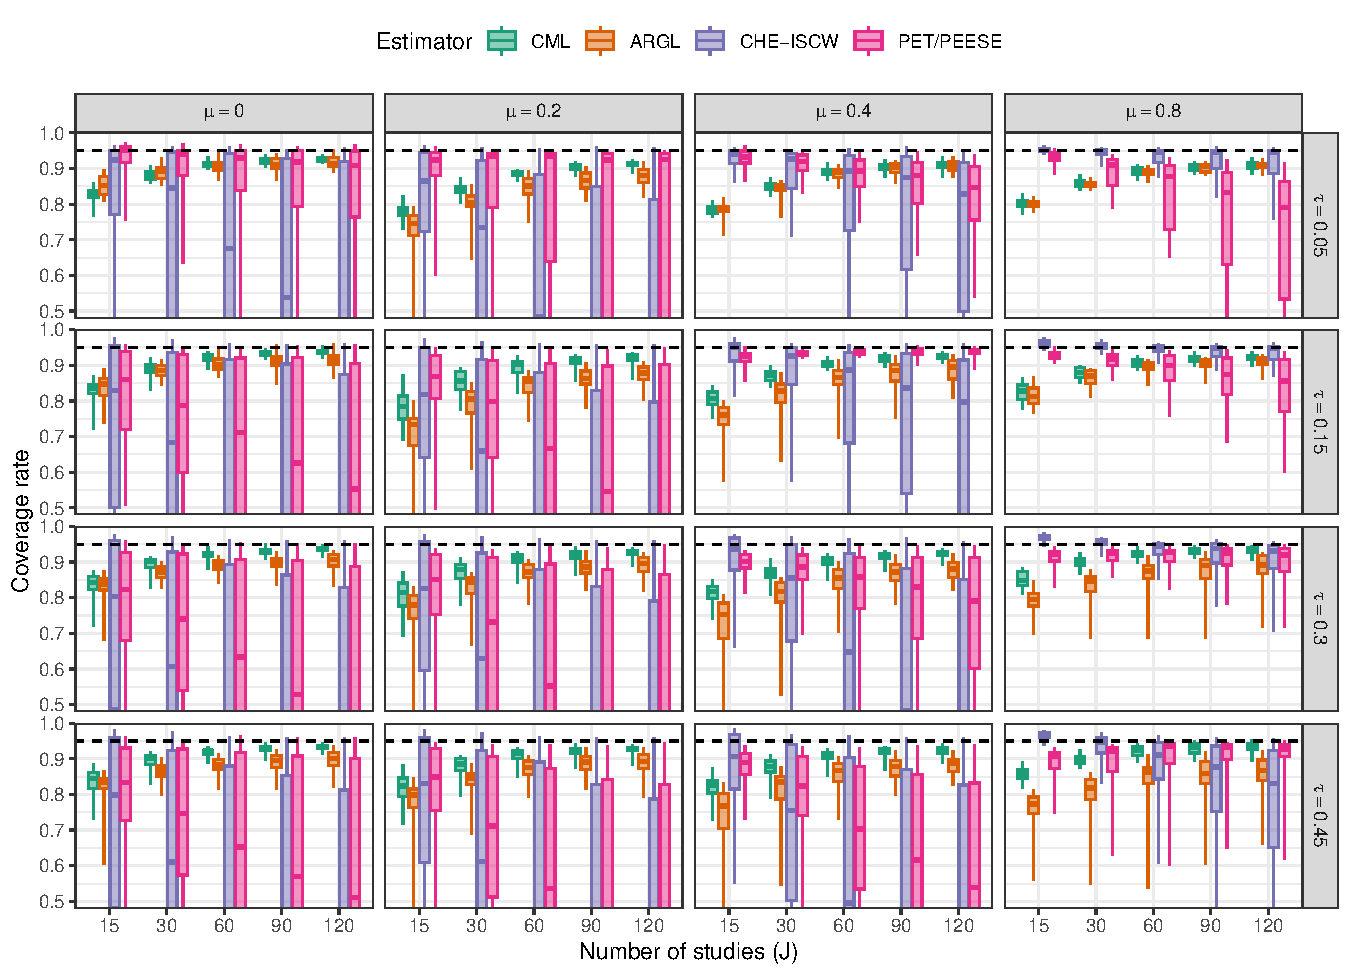
\includegraphics{step-function-selection-models-with-dependent-effects_files/figure-latex/comparison-coverage-1} \caption{Coverage levels of confidence intervals based for average effect size based on cluster-robust variance approximations, by number of studies, average SMD, and between-study heterogeneity. Dashed lines correspond to the nominal confidence level of 0.95. Coverage rates of the CHE-ISCW and PET/PEESE intervals are not depicted when they fall below 0.5}\label{fig:comparison-coverage}
\end{sidewaysfigure}

Bootstrap intervals for the step-function model provide more accurate coverage levels.
Due to the computational demands of bootstrapping, we evaluated the bootstrap confidence intervals under a more limited range of data-generating conditions, including a maximum sample size of \(J = 60\).
Figure \ref{fig:CML-coverage} depicts the coverage levels of confidence intervals based on the CML estimator, including intervals based on large-sample cluster-robust variance methods and percentile intervals using either two-stage, multinomial, or exponential (fractional reweighted) bootstrap resampling.
Although none of the intervals provide exactly nominal coverage, all versions of the percentile bootstrap intervals have coverage that is closer to nominal than the intervals based on cluster-robust variance estimation.
The percentile intervals with two-stage clustered bootstrap re-sampling provided the best coverage levels, exceeding 90\% coverage across nearly all data-generating conditions, even with only \(J = 15\) primary studies per meta-analysis.
Coverage levels of the other bootstrap intervals, including studentized, basic, and BCa intervals, were not as accurate as percentile intervals (see Supplementary Figures \ref{fig:CML-coverage-two-stage}-\ref{fig:CML-coverage-exponential} for detailed results).
Coverage levels of intervals based on the ARGL estimator followed very similar patterns to those for the CML estimator (Supplementary Figures \ref{fig:ARGL-coverage-two-stage}-\ref{fig:ARGL-coverage-exponential}).

\begin{sidewaysfigure}
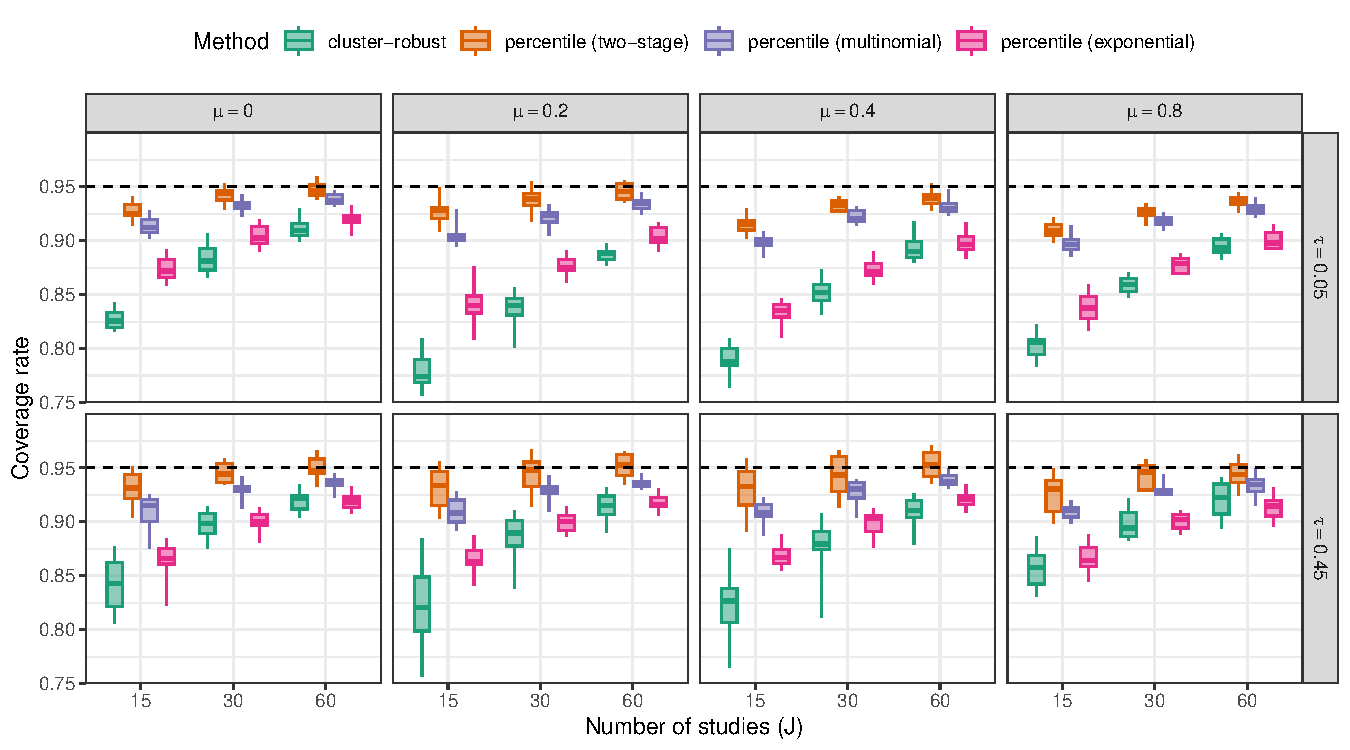
\includegraphics{step-function-selection-models-with-dependent-effects_files/figure-latex/CML-coverage-1} \caption{Coverage levels of confidence intervals based on the CML estimator of average effect size by number of studies, average SMD, and between-study heterogeneity. Dashed lines correspond to the nominal confidence level of 0.95.}\label{fig:CML-coverage}
\end{sidewaysfigure}

\section{Discussion}\label{discussion}

We have described and evaluated several methods for estimating step-function selection models while accounting for dependent effect sizes, a common feature of meta-analyses in social science fields.
We focused on the step-function selection model because it offers a number of advantages over other available methods for diagnosing and correcting selective reporting bias.
First, step-function models are generative, in that they include parameters describing the selective reporting process under simple yet plausible forms of selective reporting connected to statistical significance.
In contrast, regression-based estimators such as PET/PEESE\textsuperscript{20} or the endogenous kink meta-regression\textsuperscript{21} are agnostic as to selection mechanisms and thus are only indirectly informative about the strength or form of selection.
The step-function model also embeds a familiar evidence-generating model that allows for heterogeneity of effects through inclusion of random effects and predictors of average effect size (i.e., meta-regression).@vevea1995general
In contrast, well-known methods such as trim-and-fill\textsuperscript{18,19} and more recent proposals such as \(p\)-curve\textsuperscript{74} and \(p\)-uniform\textsuperscript{75,76} are not as flexible and have been found to perform poorly when effects are heterogeneous\textsuperscript{2}.

We treated the step-function model as a description of the \emph{marginal} distribution of the effect size estimates, effectively ignoring the dependence structure for purposes of estimating the model but accounting for it using cluster-robust sandwich estimation or clustered bootstrap inference.
This strategy is appealing for its feasibility and because it connects to a selection process in which each individual effect size is selected on the basis of its statistical significance.
We also studied two estimation methods for the marginal step-function model, composite marginal likelihood estimation and augmented-and-reweighted Gaussian likelihood estimation, and two inference strategies, based on either cluster-robust sandwich estimators or clustered bootstrap resampling.

Our simulations examined how well these estimators and inference techniques perform for recovering the average effect size under a selection process with a single step (at \(\alpha_1 = .025\)), compared to an estimator that accounts for dependence but not selection (i.e., the CHE-ISCW model) and to a variant of PET/PEESE that uses RVE.
Across an broad range of conditions, we found that both estimators of the marginal step-function model show little bias overall and consistently out-perform PET/PEESE and CHE-ISCW under conditions with meaningful selective reporting.
However, all the estimators face bias-variance trade-offs, which arise because the CHE-ISCW estimator (which does not directly adjust for selection) is substantially biased by selective reporting, whereas the CML and ARGL estimators have at most small biases.
Under conditions where selection is absent or small and where average effect size is larger, the CHE-ISCW estimator has greater precision than the estimators that adjust for selective reporting.
Because selective reporting does not create much bias under such conditions, the additional variability that comes with estimating a selection model or PET/PEESE adjustment dominates the small reduction in bias that these methods provide.
As a result, the step-function estimators are less accurate than the CHE-ISCW estimator under conditions where selective reporting is not strong or does not create meaningful bias.

The simulation results also demonstrated that the marginal step-function model estimators have better confidence interval coverage compared to the other methods, with coverage rates of the two-stage bootstrapped percentile confidence intervals approaching the nominal level of 0.95 for moderate sample sizes.
Compared to the ARGL estimator, the CML estimator of the marginal mean is usually more accurate and had confidence interval coverage rates closer to nominal levels, although differences are fairly small.
CML consistently out-performs ARGL for estimating between-study heterogeneity and the strength of selective reporting.

\subsection{Limitations and Future Directions}\label{limitations-and-future-directions}

Our approach of modeling the marginal distribution of effect sizes was motivated by the computational tractability of marginal models and by findings from prior simulations showing that univariate selection models perform well relative to alternative regression-based models to adjust for selective reporting bias.\textsuperscript{49}
However, this approach has several conceptual limitations that are important to note.
First, such models do not reflect the structure of dependence among effect size estimates drawn from the same sample, but instead describe only the overall average and overall degree of heterogeneity of the effect size distribution.
Because of this, they do not fully align with contemporary approaches for meta-analysis, which emphasize modeling the hierarchical structure of dependent effect sizes\textsuperscript{40,42}.
Second, focusing on the marginal distribution likely entails some loss of precision in parameter estimates.
Better accounting for the dependence structure, such as through the use of analytic weights, might allow for construction of more efficient estimators of the parameters of the evidence-generating process.
Third, the marginal model provides no way to distinguish between study-level publication bias and effect-level selective outcome reporting.
This strategy therefore precludes examination of more nuanced forms of selection, such as one where the probability that a given effect size is reported depends on the significance levels of other effect size estimates drawn from the same sample or on some broader feature of the study's results.

In addition to conceptual limitations, our simulation findings also need to be interpreted cautiously in light of the study's scope limitations.
First, although our simulations covered a wide range of plausible conditions, the results remain generalizable only to the data-generating process examined.
Of particular note, we generated data following a CHE effects model with primary study sample sizes and the number of effect sizes per study drawn from an empirical distribution of educational research studies.
The performance of the step-function selection models and alternative selective reporting adjustments could change based on features of studies included in the synthesis, such as studies drawn from research areas that use smaller or larger samples or that tend to assess a smaller or larger number of outcomes.
Likewise, there remains a need to investigate the robustness of the models to other evidence-generating processes, such as non-normal random effects distributions\textsuperscript{77}.

Second, the simulations examined the step-function selection model using a selection process that was compatible with the assumed model, in which the probability that an effect size was reported followed a step function in the one-sided \emph{p}-value with a threshold at \(\alpha_1 = .025\).
Other simulation studies have shown that a one-step model can be more accurate than a more complex two-step model, even when the true data-generating process aligns with the latter model.@chen2024adapting
It may require a large number of primary studies to feasibly estimate models that include multiple steps in the selection function.
Nonetheless, there may be meta-analytic datasets where a more complex set of steps is more appropriate, such as when the data include a substantial number of negative effect size estimates.

Third and related to the previous point, the simulations were limited to evidence-generating processes that did not involve systematic predictors of the effect size distribution and where the strength of selective reporting was uniform and solely dependent on the p-value of each individual effect size.
Other factors besides statistical significance of findings might affect a study's publication status.
For instance, results from pre-registered replication studies might be insulated from selective reporting or subject to different reporting pressures than other forms of primary research\textsuperscript{78}.
Further evaluation of the CML and ARGL estimators is warranted to assess their performance in models involving moderators and their robustness to other selection mechanisms.
In further development of step-function selection models, it may prove useful to model variation in the strength of reporting as a function of study characteristics such as pre-registration status\textsuperscript{79}.

Fourth and finally, the simulation findings we have reported here focused mostly on the performance of the estimators and confidence intervals for the overall average effect size, heterogeneity parameter, and selection parameter.
We have not directly evaluated how well the estimators work as diagnostic \emph{tests} for the presence of selective reporting of study results, although the below-nominal coverage rates of confidence intervals for the selection parameter suggests that they may not work well diagnostically.
In univariate random effects models, likelihood ratio tests based on step-function selection models have been found to provide much stronger power for detecting selective reporting compared to alternatives such as Egger's regression or non-parametric symmetry tests\textsuperscript{17}.
Extension of such tests for meta-analyses of dependent effect sizes requires further development.

\subsection{Conclusions}\label{conclusions}

Selective reporting of positive, statistically significant findings in primary studies can potentially distort the results of meta-analyses.
Detecting and adjusting for this form of bias is notoriously challenging---even in the simple setting where each sample contributes no more than a single effect size estimate.
These challenges are amplified with more complex data structures where the same study contributes multiple dependent effects.
Nonetheless, meta-analysts must critically evaluate the evidence summarized in a synthesis, and this includes weighing the potential for bias from selective reporting and selective publication of primary study findings.

Based on the simulation results we have presented, we recommend using step function selection models with clustered bootstrap confidence intervals to assess selective reporting bias in syntheses of dependent effect sizes. As a parametric model built on specific assumptions about the selection process, the marginal step function model provides a useful complement to more agnostic techniques for identifying small-study effects, such as funnel plots and regression adjustment methods, the bias and accuracy of which are quite variable across data-generating processes. Likewise, estimated step function models could inform the use of sensitivity analysis\textsuperscript{46} by using estimates of the strength of selection to guide assumptions about the maximal plausible degree of selection.

Consistent with recommendations from past work in the context of independent effect sizes\textsuperscript{2,80}, interpretation of any bias-corrected effect estimates needs to give consideration to the conditions under which the estimation method could be expected to perform well.
Interpretation of marginal step-function models should focus mostly on the bias-adjusted average effect size, and selection parameter estimates should be interpreted cautiously in light of the mis-calibrated coverage levels of their cluster bootstrapped confidence intervals.
More broadly, when applying and interpreting step function models, meta-analysts must consider the context of the evidence included in the synthesis, such as whether the effect size estimates are for focal results or merely incidental findings and whether studies were conducted under conditions where pressures to selectively reporting findings are present.
As with inferences from any model, one's conclusions should be informed not only by the statistical results but also by knowledge of the research context.

\section*{Author Contributions}\label{author-contributions}
\addcontentsline{toc}{section}{Author Contributions}

\textbf{JEP:} Conceptualization, Methodology, Software, Validation, Formal Analysis, Investigation, Resources, Writing - original draft, Writing - review \& editing, Supervision \textbf{MJ:} Methodology, Software, Validation, Formal Analysis, Investigation, Writing - original draft, Writing - review \& editing, Visualization \textbf{MC:} Conceptualization, Methodology, Investigation, Writing - original draft, Writing - review \& editing, Project administration, Funding acquisition

\section*{Funding}\label{funding}
\addcontentsline{toc}{section}{Funding}

This work was supported, in part, by the Institute of Educational Sciences, U.S. Department of Education through grant R305D220026 to the American Institutes of Research.
The opinions expressed are those of the authors and do not represent the views of the Institute of the U.S. Department of Education.

\section*{Acknowledgements}\label{acknowledgements}
\addcontentsline{toc}{section}{Acknowledgements}

We thank Laura Michaelson for feedback on a draft version of this article.

\section*{Data and Replication Materials}\label{data-and-replication-materials}
\addcontentsline{toc}{section}{Data and Replication Materials}

Code and data for replicating the empirical example and the Monte Carlo simulation study are available on the Open Science Framework at \url{https://osf.io/v25rx/}.

\section*{Conflict of Interest Statement}\label{conflict-of-interest-statement}
\addcontentsline{toc}{section}{Conflict of Interest Statement}

The authors declare no conflicts of interest.

\section*{References}\label{references}
\addcontentsline{toc}{section}{References}

\begingroup
\singlespacing
\setlength{\parindent}{-0.5in}
\setlength{\leftskip}{0.5in}

\protect\phantomsection\label{refs}
\begin{CSLReferences}{0}{1}
\bibitem[\citeproctext]{ref-Rothstein2005publication}
\CSLLeftMargin{1. }%
\CSLRightInline{Rothstein HR, Sutton AJ, Borenstein M. Publication bias in meta-analysis. In: Rothstein HR, Sutton AJ, Borenstein M, eds. \emph{Publication {Bias} in {Meta-Analysis}: {Prevention}, {Assessment}, and {Adjustments}}. {John Wiley \& Sons}; 2005:1-7. doi:\href{https://doi.org/10.1002/0470870168}{10.1002/0470870168}}

\bibitem[\citeproctext]{ref-carter2019correcting}
\CSLLeftMargin{2. }%
\CSLRightInline{Carter EC, Schönbrodt FD, Gervais WM, Hilgard J. Correcting for bias in psychology: A comparison of meta-analytic methods. \emph{Advances in Methods and Practices in Psychological Science}. 2019;2(2):115-144.}

\bibitem[\citeproctext]{ref-chan2004empirical}
\CSLLeftMargin{3. }%
\CSLRightInline{Chan AW, Hróbjartsson A, Haahr MT, Gøtzsche PC, Altman DG. Empirical evidence for selective reporting of outcomes in randomized trials: Comparison of protocols to published articles. \emph{Jama}. 2004;291(20):2457-2465.}

\bibitem[\citeproctext]{ref-pigott2013outcome}
\CSLLeftMargin{4. }%
\CSLRightInline{Pigott TD, Valentine JC, Polanin JR, Williams RT, Canada DD. Outcome-reporting bias in education research. \emph{Educational Researcher}. 2013;42(8):424-432.}

\bibitem[\citeproctext]{ref-lancee2017outcome}
\CSLLeftMargin{5. }%
\CSLRightInline{Lancee M, Lemmens C, Kahn R, Vinkers C, Luykx J. Outcome reporting bias in randomized-controlled trials investigating antipsychotic drugs. \emph{Translational psychiatry}. 2017;7(9):e1232-e1232.}

\bibitem[\citeproctext]{ref-john2012measuring}
\CSLLeftMargin{6. }%
\CSLRightInline{John LK, Loewenstein G, Prelec D. Measuring the prevalence of questionable research practices with incentives for truth telling. \emph{Psychological science}. 2012;23(5):524-532.}

\bibitem[\citeproctext]{ref-franco2016underreporting}
\CSLLeftMargin{7. }%
\CSLRightInline{Franco A, Malhotra N, Simonovits G. Underreporting in psychology experiments: Evidence from a study registry. \emph{Social Psychological and Personality Science}. 2016;7(1):8-12. doi:\href{https://doi.org/10.1177/1948550615598377}{10.1177/1948550615598377}}

\bibitem[\citeproctext]{ref-oBoyle2017chrysalis}
\CSLLeftMargin{8. }%
\CSLRightInline{O'Boyle Jr EH, Banks GC, Gonzalez-Mulé E. The chrysalis effect: How ugly initial results metamorphosize into beautiful articles. \emph{Journal of Management}. 2017;43(2):376-399.}

\bibitem[\citeproctext]{ref-marksanglin2020historical}
\CSLLeftMargin{9. }%
\CSLRightInline{Marks‐Anglin A, Chen Y. A historical review of publication bias. \emph{Res Syn Meth}. 2020;11(6):725-742. doi:\href{https://doi.org/10.1002/jrsm.1452}{10.1002/jrsm.1452}}

\bibitem[\citeproctext]{ref-light1984Summing}
\CSLLeftMargin{10. }%
\CSLRightInline{Light RJ, Pillemer DB. \emph{Summing {Up}}. {Harvard University Press}; 1984. \url{https://books.google.com?id=qel3lAm4K6gC}}

\bibitem[\citeproctext]{ref-Sterne2005funnel}
\CSLLeftMargin{11. }%
\CSLRightInline{Sterne JAC, Becker BJ, Egger M. The funnel plot. In: Rothstein HR, Sutton AJ, Borenstein M, eds. \emph{Publication {Bias} in {Meta-Analysis}: {Prevention}, {Assessment}, and {Adjustments}}. {John Wiley \& Sons}; 2005:73-98. doi:\href{https://doi.org/10.1002/0470870168}{10.1002/0470870168}}

\bibitem[\citeproctext]{ref-kossmeier2020PowerEnhanced}
\CSLLeftMargin{12. }%
\CSLRightInline{Kossmeier M, Tran US, Voracek M. Power-enhanced funnel plots for meta-analysis. \emph{Zeitschrift für Psychologie}. Published online March 31, 2020. \url{https://econtent.hogrefe.com/doi/10.1027/2151-2604/a000392}}

\bibitem[\citeproctext]{ref-begg1994operating}
\CSLLeftMargin{13. }%
\CSLRightInline{Begg CB, Mazumdar M. Operating characteristics of a rank correlation test for publication bias. \emph{Biometrics}. Published online 1994:1088-1101.}

\bibitem[\citeproctext]{ref-egger1997bias}
\CSLLeftMargin{14. }%
\CSLRightInline{Egger M, Smith GD, Schneider M, Minder C. Bias in meta-analysis detected by a simple, graphical test. \emph{BMJ}. 1997;315(7109):629-634.}

\bibitem[\citeproctext]{ref-harbord2006modified}
\CSLLeftMargin{15. }%
\CSLRightInline{Harbord RM, Egger M, Sterne JA. A modified test for small-study effects in meta-analyses of controlled trials with binary endpoints. \emph{Statistics in medicine}. 2006;25(20):3443-3457.}

\bibitem[\citeproctext]{ref-moreno2012generalized}
\CSLLeftMargin{16. }%
\CSLRightInline{Moreno SG, Sutton AJ, Thompson JR, Ades A, Abrams KR, Cooper NJ. A generalized weighting regression-derived meta-analysis estimator robust to small-study effects and heterogeneity. \emph{Statistics in medicine}. 2012;31(14):1407-1417.}

\bibitem[\citeproctext]{ref-pustejovsky2019testing}
\CSLLeftMargin{17. }%
\CSLRightInline{Pustejovsky JE, Rodgers MA. Testing for funnel plot asymmetry of standardized mean differences. \emph{Research Synthesis Methods}. 2019;10(1):57-71.}

\bibitem[\citeproctext]{ref-duval2000nonparametric}
\CSLLeftMargin{18. }%
\CSLRightInline{Duval S, Tweedie R. A nonparametric {``trim and fill''} method of accounting for publication bias in meta-analysis. \emph{Journal of the american statistical association}. 2000;95(449):89-98.}

\bibitem[\citeproctext]{ref-duval2000trim}
\CSLLeftMargin{19. }%
\CSLRightInline{Duval S, Tweedie R. Trim and fill: A simple funnel-plot--based method of testing and adjusting for publication bias in meta-analysis. \emph{Biometrics}. 2000;56(2):455-463.}

\bibitem[\citeproctext]{ref-stanley2014meta}
\CSLLeftMargin{20. }%
\CSLRightInline{Stanley TD, Doucouliagos H. Meta-regression approximations to reduce publication selection bias. \emph{Research Synthesis Methods}. 2014;5(1):60-78.}

\bibitem[\citeproctext]{ref-bom2019kinked}
\CSLLeftMargin{21. }%
\CSLRightInline{Bom PRD, Rachinger H. A kinked meta-regression model for publication bias correction. \emph{Research Synthesis Methods}. 2019;10(4):497-514. doi:\href{https://doi.org/10.1002/jrsm.1352}{10.1002/jrsm.1352}}

\bibitem[\citeproctext]{ref-hedges1984estimation}
\CSLLeftMargin{22. }%
\CSLRightInline{Hedges LV. Estimation of effect size under nonrandom sampling: The effects of censoring studies yielding statistically insignificant mean differences. \emph{Journal of Educational Statistics}. 1984;9(1):61-85.}

\bibitem[\citeproctext]{ref-iyengar1988selection}
\CSLLeftMargin{23. }%
\CSLRightInline{Iyengar S, Greenhouse JB. Selection {Models} and the {File} {Drawer} {Problem}. \emph{Statistical Science}. 1988;3(1):109-117. doi:\href{https://doi.org/10.1214/ss/1177013012}{10.1214/ss/1177013012}}

\bibitem[\citeproctext]{ref-dear1992approach}
\CSLLeftMargin{24. }%
\CSLRightInline{Dear KBG, Begg CB. {An approach for assessing publication bias prior to performing a meta-analysis}. \emph{Statistical Science}. 1992;7(2):237-245.}

\bibitem[\citeproctext]{ref-hedges1992modeling}
\CSLLeftMargin{25. }%
\CSLRightInline{Hedges LV. Modeling publication selection effects in meta-analysis. \emph{Statistical Science}. 1992;7(2):246-255.}

\bibitem[\citeproctext]{ref-vevea1995general}
\CSLLeftMargin{26. }%
\CSLRightInline{Vevea JL, Hedges LV. A general linear model for estimating effect size in the presence of publication bias. \emph{Psychometrika}. 1995;60(3):419-435. doi:\href{https://doi.org/10.1007/BF02294384}{10.1007/BF02294384}}

\bibitem[\citeproctext]{ref-citkowicz2017parsimonious}
\CSLLeftMargin{27. }%
\CSLRightInline{Citkowicz M, Vevea JL. {A parsimonious weight function for modeling publication bias}. \emph{Psychological Methods}. 2017;22(1):28-41. doi:\href{https://doi.org/10.1037/met0000119}{10.1037/met0000119}}

\bibitem[\citeproctext]{ref-preston2004adjusting}
\CSLLeftMargin{28. }%
\CSLRightInline{Preston C, Ashby D, Smyth R. Adjusting for publication bias: Modelling the selection process. \emph{Evaluation Clinical Practice}. 2004;10(2):313-322. doi:\href{https://doi.org/10.1111/j.1365-2753.2003.00457.x}{10.1111/j.1365-2753.2003.00457.x}}

\bibitem[\citeproctext]{ref-Terrin2003heterogeneity}
\CSLLeftMargin{29. }%
\CSLRightInline{Terrin N, Schmid CH, Lau J, Olkin I. Adjusting for publication bias in the presence of heterogeneity. \emph{Statistics in Medicine}. 2003;22(13):2113-2126. doi:\href{https://doi.org/10.1002/sim.1461}{10.1002/sim.1461}}

\bibitem[\citeproctext]{ref-greenwald1975prejudice}
\CSLLeftMargin{30. }%
\CSLRightInline{Greenwald AG. Consequences of prejudice against the null hypothesis. \emph{Psychological Bulletin}. 1975;82(1):1-20. doi:\href{https://doi.org/10.1037/h0076157}{10.1037/h0076157}}

\bibitem[\citeproctext]{ref-Nelson1986significance}
\CSLLeftMargin{31. }%
\CSLRightInline{Nelson N, Rosenthal R, Rosnow RL. Interpretation of significance levels and effect sizes by psychological researchers. \emph{American Psychologist}. 1986;41(11):1299-1301. doi:\href{https://doi.org/10.1037/0003-066X.41.11.1299}{10.1037/0003-066X.41.11.1299}}

\bibitem[\citeproctext]{ref-Rosenthal1963significance}
\CSLLeftMargin{32. }%
\CSLRightInline{Rosenthal R, Gaito J. The interpretation of levels of significance by psychological researchers. \emph{The Journal of Psychology: Interdisciplinary and Applied}. 1963;55(1):33-38. doi:\href{https://doi.org/10.1080/00223980.1963.9916596}{10.1080/00223980.1963.9916596}}

\bibitem[\citeproctext]{ref-Rosenthal1964significance}
\CSLLeftMargin{33. }%
\CSLRightInline{Rosenthal R, Gaito J. Further evidence for the cliff effect in the interpretation of levels of significance. \emph{Psychological Reports}. 1964;15(2):570. doi:\href{https://doi.org/10.2466/pr0.1964.15.2.570}{10.2466/pr0.1964.15.2.570}}

\bibitem[\citeproctext]{ref-Becker2000multivariate}
\CSLLeftMargin{34. }%
\CSLRightInline{Becker BJ. {Multivariate Meta-analysis}. In: Brown SD, Tinsley HEA, eds. \emph{Handbook of Applied Multivariate Statistics and Mathematical Modeling}. Academic Press; 2000:499-525. doi:\href{https://doi.org/10.1016/B978-012691360-6/50018-5}{10.1016/B978-012691360-6/50018-5}}

\bibitem[\citeproctext]{ref-Hedges2010robust}
\CSLLeftMargin{35. }%
\CSLRightInline{Hedges LV, Tipton E, Johnson MC. {Robust variance estimation in meta-regression with dependent effect size estimates}. \emph{Research Synthesis Methods}. 2010;1(1):39-65. doi:\href{https://doi.org/10.1002/jrsm.5}{10.1002/jrsm.5}}

\bibitem[\citeproctext]{ref-tipton2019current}
\CSLLeftMargin{36. }%
\CSLRightInline{Tipton E, Pustejovsky JE, Ahmadi H. Current practices in meta-regression in psychology, education, and medicine. \emph{Research synthesis methods}. 2019;10(2):180-194.}

\bibitem[\citeproctext]{ref-nakagawa2023quantitative}
\CSLLeftMargin{37. }%
\CSLRightInline{Nakagawa S, Yang Y, Macartney EL, Spake R, Lagisz M. Quantitative evidence synthesis: A practical guide on meta-analysis, meta-regression, and publication bias tests for environmental sciences. \emph{Environ Evid}. 2023;12(1):8. doi:\href{https://doi.org/10.1186/s13750-023-00301-6}{10.1186/s13750-023-00301-6}}

\bibitem[\citeproctext]{ref-yang2023advanced}
\CSLLeftMargin{38. }%
\CSLRightInline{Yang Y, Macleod M, Pan J, Lagisz M, Nakagawa S. Advanced methods and implementations for the meta-analyses of animal models: {Current} practices and future recommendations. \emph{Neuroscience \& Biobehavioral Reviews}. 2023;146:105016. doi:\href{https://doi.org/10.1016/j.neubiorev.2022.105016}{10.1016/j.neubiorev.2022.105016}}

\bibitem[\citeproctext]{ref-konstantopoulos2011fixed}
\CSLLeftMargin{39. }%
\CSLRightInline{Konstantopoulos S. Fixed effects and variance components estimation in three-level meta-analysis: {Three}-level meta-analysis. \emph{Research Synthesis Methods}. 2011;2(1):61-76. doi:\href{https://doi.org/10.1002/jrsm.35}{10.1002/jrsm.35}}

\bibitem[\citeproctext]{ref-vandennoortgate2013threelevel}
\CSLLeftMargin{40. }%
\CSLRightInline{Van den Noortgate W, López-López JA, Marín-Martínez F, Sánchez-Meca J. Three-level meta-analysis of dependent effect sizes. \emph{Behavior Research Methods}. 2013;45(2):576-594. doi:\href{https://doi.org/10.3758/s13428-012-0261-6}{10.3758/s13428-012-0261-6}}

\bibitem[\citeproctext]{ref-vandennoortgate2015metaanalysis}
\CSLLeftMargin{41. }%
\CSLRightInline{Van den Noortgate W, López-López JA, Marín-Martínez F, Sánchez-Meca J. Meta-analysis of multiple outcomes: A multilevel approach. \emph{Behavior Research Methods}. 2015;47(4):1274-1294. doi:\href{https://doi.org/10.3758/s13428-014-0527-2}{10.3758/s13428-014-0527-2}}

\bibitem[\citeproctext]{ref-pustejovsky2022preventionscience}
\CSLLeftMargin{42. }%
\CSLRightInline{Pustejovsky JE, Tipton E. Meta-Analysis with Robust Variance Estimation: {Expanding} the Range of Working Models. \emph{Prevention Science}. 2022;23:425-438. doi:\href{https://doi.org/10.1016/j.jsp.2018.02.003}{10.1016/j.jsp.2018.02.003}}

\bibitem[\citeproctext]{ref-tipton2015small}
\CSLLeftMargin{43. }%
\CSLRightInline{Tipton E. Small sample adjustments for robust variance estimation with meta-regression. \emph{Psychological methods}. 2015;20(3):375.}

\bibitem[\citeproctext]{ref-tiptonpusto2015small}
\CSLLeftMargin{44. }%
\CSLRightInline{Tipton E, Pustejovsky JE. Small-sample adjustments for tests of moderators and model fit using robust variance estimation in meta-regression. \emph{Journal of Educational and Behavioral Statistics}. 2015;40(6):604-634.}

\bibitem[\citeproctext]{ref-joshi2022cluster}
\CSLLeftMargin{45. }%
\CSLRightInline{Joshi M, Pustejovsky JE, Beretvas SN. Cluster Wild Bootstrapping to Handle Dependent Effect Sizes in Meta-Analysis with a Small Number of Studies. \emph{Research Synthesis Methods}. 2022;13(4):457-477. doi:\href{https://doi.org/10.1002/jrsm.1554}{10.1002/jrsm.1554}}

\bibitem[\citeproctext]{ref-mathur2020sensitivity}
\CSLLeftMargin{46. }%
\CSLRightInline{Mathur MB, VanderWeele TJ. Sensitivity analysis for publication bias in meta‐analyses. \emph{J R Stat Soc C}. 2020;69(5):1091-1119. doi:\href{https://doi.org/10.1111/rssc.12440}{10.1111/rssc.12440}}

\bibitem[\citeproctext]{ref-fernandezcastilla2019detecting}
\CSLLeftMargin{47. }%
\CSLRightInline{Fernández-Castilla B, Declercq L, Jamshidi L, Beretvas SN, Onghena P, Van den Noortgate W. Detecting selection bias in meta-analyses with multiple outcomes: A simulation study. \emph{The Journal of Experimental Education}. Published online April 2019:1-20. doi:\href{https://doi.org/10.1080/00220973.2019.1582470}{10.1080/00220973.2019.1582470}}

\bibitem[\citeproctext]{ref-rodgers2021evaluating}
\CSLLeftMargin{48. }%
\CSLRightInline{Rodgers MA, Pustejovsky JE. Evaluating meta-analytic methods to detect selective reporting in the presence of dependent effect sizes. \emph{Psychological methods}. 2021;26(2):141.}

\bibitem[\citeproctext]{ref-chen2024adapting}
\CSLLeftMargin{49. }%
\CSLRightInline{Chen M, Pustejovsky JE. Adapting methods for correcting selective reporting bias in meta-analysis of dependent effect sizes. Published online October 23, 2024. doi:\href{https://doi.org/10.31222/osf.io/jq52s}{10.31222/osf.io/jq52s}}

\bibitem[\citeproctext]{ref-hedges2005selection}
\CSLLeftMargin{50. }%
\CSLRightInline{Hedges LV, Vevea J. Selection method approaches. In: Rothstein HR, Sutton AJ, Borenstein M, eds. \emph{Publication Bias in Meta-Analysis}. {John Wiley \& Sons, Ltd}; 2005:145-174. doi:\href{https://doi.org/10.1002/0470870168.ch9}{10.1002/0470870168.ch9}}

\bibitem[\citeproctext]{ref-vevea2005publication}
\CSLLeftMargin{51. }%
\CSLRightInline{Vevea JL, Woods CM. Publication bias in research synthesis: Sensitivity analysis using a priori weight functions. \emph{Psychological Methods}. 2005;10(4):428-443. doi:\href{https://doi.org/10.1037/1082-989X.10.4.428}{10.1037/1082-989X.10.4.428}}

\bibitem[\citeproctext]{ref-cox2004note}
\CSLLeftMargin{52. }%
\CSLRightInline{Cox DR, Reid N. A note on pseudolikelihood constructed from marginal densities. \emph{Biometrika}. 2004;91(3):729-737. doi:\href{https://doi.org/10.1093/biomet/91.3.729}{10.1093/biomet/91.3.729}}

\bibitem[\citeproctext]{ref-lindsay1988composite}
\CSLLeftMargin{53. }%
\CSLRightInline{Lindsay BG. Composite likelihood methods. In: Prabhu NU, ed. \emph{Contemporary {Mathematics}}. Vol 80. American Mathematical Society; 1988:221-239. doi:\href{https://doi.org/10.1090/conm/080/999014}{10.1090/conm/080/999014}}

\bibitem[\citeproctext]{ref-varin2008composite}
\CSLLeftMargin{54. }%
\CSLRightInline{Varin C. On composite marginal likelihoods. \emph{AStA}. 2008;92(1):1-28. doi:\href{https://doi.org/10.1007/s10182-008-0060-7}{10.1007/s10182-008-0060-7}}

\bibitem[\citeproctext]{ref-davison1997bootstrap}
\CSLLeftMargin{55. }%
\CSLRightInline{Davison AC, Hinkley DV. \emph{Bootstrap Methods and Their Applications}. Cambridge University Press; 1997.}

\bibitem[\citeproctext]{ref-field2007bootstrapping}
\CSLLeftMargin{56. }%
\CSLRightInline{Field CA, Welsh AH. Bootstrapping clustered data. \emph{Journal of the Royal Statistical Society Series B: Statistical Methodology}. 2007;69(3):369-390. doi:\href{https://doi.org/10.1111/j.1467-9868.2007.00593.x}{10.1111/j.1467-9868.2007.00593.x}}

\bibitem[\citeproctext]{ref-leeuw2008resampling}
\CSLLeftMargin{57. }%
\CSLRightInline{Leeden RVD, Meijer E, Busing FMTA. Resampling multilevel models. In: Leeuw JD, Meijer E, eds. \emph{Handbook of {Multilevel} {Analysis}}. Springer New York; 2008:401-433. doi:\href{https://doi.org/10.1007/978-0-387-73186-5_11}{10.1007/978-0-387-73186-5\_11}}

\bibitem[\citeproctext]{ref-xu2020applications}
\CSLLeftMargin{58. }%
\CSLRightInline{Xu L, Gotwalt C, Hong Y, King CB, Meeker WQ. Applications of the fractional-random-weight bootstrap. \emph{The American Statistician}. 2020;74(4):345-358. doi:\href{https://doi.org/10.1080/00031305.2020.1731599}{10.1080/00031305.2020.1731599}}

\bibitem[\citeproctext]{ref-efron1987better}
\CSLLeftMargin{59. }%
\CSLRightInline{Efron B. Better bootstrap confidence intervals. \emph{Journal of the American Statistical Association}. 1987;82(397):171-185. doi:\href{https://doi.org/10.1080/01621459.1987.10478410}{10.1080/01621459.1987.10478410}}

\bibitem[\citeproctext]{ref-carter2015series}
\CSLLeftMargin{60. }%
\CSLRightInline{Carter EC, Kofler LM, Forster DE, McCullough ME. A series of meta-analytic tests of the depletion effect: Self-control does not seem to rely on a limited resource. \emph{Journal of Experimental Psychology: General}. 2015;144(4):796.}

\bibitem[\citeproctext]{ref-hagger2010ego}
\CSLLeftMargin{61. }%
\CSLRightInline{Hagger MS, Wood C, Stiff C, Chatzisarantis NLD. Ego depletion and the strength model of self-control: {A} meta-analysis. \emph{Psychological Bulletin}. 2010;136(4):495-525. doi:\href{https://doi.org/10.1037/a0019486}{10.1037/a0019486}}

\bibitem[\citeproctext]{ref-rcoreteam}
\CSLLeftMargin{62. }%
\CSLRightInline{R Core Team. \emph{R: A Language and Environment for Statistical Computing}. R Foundation for Statistical Computing; 2025. \url{https://www.R-project.org/}}

\bibitem[\citeproctext]{ref-metaselection}
\CSLLeftMargin{63. }%
\CSLRightInline{Pustejovsky JE, Joshi M, Citkowicz M. \emph{Metaselection: Meta-Analytic Selection Models with Cluster-Robust and Cluster-Bootstrap Standard Errors for Dependent Effect Size Estimates}.; 2025. \url{https://github.com/jepusto/metaselection}}

\bibitem[\citeproctext]{ref-CHTC}
\CSLLeftMargin{64. }%
\CSLRightInline{Center for High Throughput Computing. Center for high throughput computing. Published online 2006. doi:\href{https://doi.org/10.21231/GNT1-HW21}{10.21231/GNT1-HW21}}

\bibitem[\citeproctext]{ref-Viechtbauer2010conducting}
\CSLLeftMargin{65. }%
\CSLRightInline{Viechtbauer W. {Conducting meta-analyses in R with the metafor package}. \emph{Journal of Statistical Software}. 2010;36(3):1-48.}

\bibitem[\citeproctext]{ref-clubSandwich}
\CSLLeftMargin{66. }%
\CSLRightInline{Pustejovsky JE. \emph{clubSandwich: Cluster-Robust (Sandwich) Variance Estimators with Small-Sample Corrections}.; 2024. \url{https://CRAN.R-project.org/package=clubSandwich}}

\bibitem[\citeproctext]{ref-simhelpers}
\CSLLeftMargin{67. }%
\CSLRightInline{Joshi M, Pustejovsky JE. \emph{Simhelpers: Helper Functions for Simulation Studies}.; 2024. \url{https://meghapsimatrix.github.io/simhelpers/}}

\bibitem[\citeproctext]{ref-optimx}
\CSLLeftMargin{68. }%
\CSLRightInline{Nash JC, Varadhan R. Unifying optimization algorithms to aid software system users: {optimx} for {R}. \emph{Journal of Statistical Software}. 2011;43(9):1-14. doi:\href{https://doi.org/10.18637/jss.v043.i09}{10.18637/jss.v043.i09}}

\bibitem[\citeproctext]{ref-nleqslv}
\CSLLeftMargin{69. }%
\CSLRightInline{Hasselman B. \emph{Nleqslv: Solve Systems of Nonlinear Equations}.; 2023. \url{https://CRAN.R-project.org/package=nleqslv}}

\bibitem[\citeproctext]{ref-tidyverse}
\CSLLeftMargin{70. }%
\CSLRightInline{Wickham H, Averick M, Bryan J, et al. Welcome to the {tidyverse}. \emph{Journal of Open Source Software}. 2019;4(43):1686. doi:\href{https://doi.org/10.21105/joss.01686}{10.21105/joss.01686}}

\bibitem[\citeproctext]{ref-borenstein2019effect}
\CSLLeftMargin{71. }%
\CSLRightInline{Borenstein M, Hedges LV. Effect sizes for meta-analysis. \emph{The handbook of research synthesis and meta-analysis}. 2019;3:207-243.}

\bibitem[\citeproctext]{ref-kraft2020interpreting}
\CSLLeftMargin{72. }%
\CSLRightInline{Kraft MA. Interpreting effect sizes of education interventions. \emph{Educational researcher}. 2020;49(4):241-253.}

\bibitem[\citeproctext]{ref-boos2000montecarlo}
\CSLLeftMargin{73. }%
\CSLRightInline{Boos DD, Zhang J. Monte carlo evaluation of resampling-based hypothesis tests. \emph{Journal of the American Statistical Association}. 2000;95(450):486-492. doi:\href{https://doi.org/10.1080/01621459.2000.10474226}{10.1080/01621459.2000.10474226}}

\bibitem[\citeproctext]{ref-simonsohn2014pcurve}
\CSLLeftMargin{74. }%
\CSLRightInline{Simonsohn U, Nelson LD, Simmons JP. P-curve and effect size: Correcting for publication bias using only significant results. \emph{Perspectives on Psychological Science}. 2014;9(6):666-681. doi:\href{https://doi.org/10.1177/1745691614553988}{10.1177/1745691614553988}}

\bibitem[\citeproctext]{ref-VanAssen2015meta}
\CSLLeftMargin{75. }%
\CSLRightInline{Assen MALM van, Van Aert RCM, Wicherts JM. {Meta-analysis using effect size distributions of only statistically significant studies}. \emph{Psychological Methods}. 2015;20(3):293-309. doi:\url{http://dx.doi.org/10.1037/met0000025}}

\bibitem[\citeproctext]{ref-vanaert2016conducting}
\CSLLeftMargin{76. }%
\CSLRightInline{Aert RCM van, Wicherts JM, Assen MALM van. Conducting meta-analyses based on \emph{p} values: Reservations and recommendations for applying \emph{p} -uniform and \emph{p} -curve. \emph{Perspectives on Psychological Science}. 2016;11(5):713-729. doi:\href{https://doi.org/10.1177/1745691616650874}{10.1177/1745691616650874}}

\bibitem[\citeproctext]{ref-Hedges1996estimating}
\CSLLeftMargin{77. }%
\CSLRightInline{Hedges LV, Vevea JL. {Estimating effect size under publication bias: Small sample properties and robustness of a random effects selection model}. \emph{Journal of Educational and Behavioral Statistics}. 1996;21(4):299. doi:\href{https://doi.org/10.3102/10769986021004299}{10.3102/10769986021004299}}

\bibitem[\citeproctext]{ref-vanaert2025metaanalyzing}
\CSLLeftMargin{78. }%
\CSLRightInline{Van Aert RCM. Meta-analyzing nonpreregistered and preregistered studies. \emph{Psychological Methods}. Published online February 17, 2025. doi:\href{https://doi.org/10.1037/met0000719}{10.1037/met0000719}}

\bibitem[\citeproctext]{ref-Coburn2015publication}
\CSLLeftMargin{79. }%
\CSLRightInline{Coburn KM, Vevea JL. {Publication bias as a function of study characteristics}. \emph{Psychological Methods}. 2015;20(3):310-330. doi:\href{https://doi.org/10.1037/met0000046}{10.1037/met0000046}}

\bibitem[\citeproctext]{ref-mcshane2016adjusting}
\CSLLeftMargin{80. }%
\CSLRightInline{McShane BB, Böckenholt U, Hansen KT. Adjusting for publication bias in meta-analysis an evaluation of selection methods and some cautionary notes. \emph{Perspectives on Psychological Science}. 2016;11(5):730-749. Accessed November 1, 2016. \url{http://pps.sagepub.com/content/11/5/730.short}}

\end{CSLReferences}

\endgroup


\end{document}
